\documentclass[twoside]{book}

% Packages required by doxygen
\usepackage{fixltx2e}
\usepackage{calc}
\usepackage{doxygen}
\usepackage[export]{adjustbox} % also loads graphicx
\usepackage{graphicx}
\usepackage[utf8]{inputenc}
\usepackage{makeidx}
\usepackage{multicol}
\usepackage{multirow}
\PassOptionsToPackage{warn}{textcomp}
\usepackage{textcomp}
\usepackage[nointegrals]{wasysym}
\usepackage[table]{xcolor}

% Font selection
\usepackage[T1]{fontenc}
\usepackage[scaled=.90]{helvet}
\usepackage{courier}
\usepackage{amssymb}
\usepackage{sectsty}
\renewcommand{\familydefault}{\sfdefault}
\allsectionsfont{%
  \fontseries{bc}\selectfont%
  \color{darkgray}%
}
\renewcommand{\DoxyLabelFont}{%
  \fontseries{bc}\selectfont%
  \color{darkgray}%
}
\newcommand{\+}{\discretionary{\mbox{\scriptsize$\hookleftarrow$}}{}{}}

% Page & text layout
\usepackage{geometry}
\geometry{%
  a4paper,%
  top=2.5cm,%
  bottom=2.5cm,%
  left=2.5cm,%
  right=2.5cm%
}
\tolerance=750
\hfuzz=15pt
\hbadness=750
\setlength{\emergencystretch}{15pt}
\setlength{\parindent}{0cm}
\setlength{\parskip}{3ex plus 2ex minus 2ex}
\makeatletter
\renewcommand{\paragraph}{%
  \@startsection{paragraph}{4}{0ex}{-1.0ex}{1.0ex}{%
    \normalfont\normalsize\bfseries\SS@parafont%
  }%
}
\renewcommand{\subparagraph}{%
  \@startsection{subparagraph}{5}{0ex}{-1.0ex}{1.0ex}{%
    \normalfont\normalsize\bfseries\SS@subparafont%
  }%
}
\makeatother

% Headers & footers
\usepackage{fancyhdr}
\pagestyle{fancyplain}
\fancyhead[LE]{\fancyplain{}{\bfseries\thepage}}
\fancyhead[CE]{\fancyplain{}{}}
\fancyhead[RE]{\fancyplain{}{\bfseries\leftmark}}
\fancyhead[LO]{\fancyplain{}{\bfseries\rightmark}}
\fancyhead[CO]{\fancyplain{}{}}
\fancyhead[RO]{\fancyplain{}{\bfseries\thepage}}
\fancyfoot[LE]{\fancyplain{}{}}
\fancyfoot[CE]{\fancyplain{}{}}
\fancyfoot[RE]{\fancyplain{}{\bfseries\scriptsize Generated by Doxygen }}
\fancyfoot[LO]{\fancyplain{}{\bfseries\scriptsize Generated by Doxygen }}
\fancyfoot[CO]{\fancyplain{}{}}
\fancyfoot[RO]{\fancyplain{}{}}
\renewcommand{\footrulewidth}{0.4pt}
\renewcommand{\chaptermark}[1]{%
  \markboth{#1}{}%
}
\renewcommand{\sectionmark}[1]{%
  \markright{\thesection\ #1}%
}

% Indices & bibliography
\usepackage{natbib}
\usepackage[titles]{tocloft}
\setcounter{tocdepth}{3}
\setcounter{secnumdepth}{5}
\makeindex

% Hyperlinks (required, but should be loaded last)
\usepackage{ifpdf}
\ifpdf
  \usepackage[pdftex,pagebackref=true]{hyperref}
\else
  \usepackage[ps2pdf,pagebackref=true]{hyperref}
\fi
\hypersetup{%
  colorlinks=true,%
  linkcolor=blue,%
  citecolor=blue,%
  unicode%
}

% Custom commands
\newcommand{\clearemptydoublepage}{%
  \newpage{\pagestyle{empty}\cleardoublepage}%
}

\usepackage{caption}
\captionsetup{labelsep=space,justification=centering,font={bf},singlelinecheck=off,skip=4pt,position=top}

%===== C O N T E N T S =====

\begin{document}

% Titlepage & ToC
\hypersetup{pageanchor=false,
             bookmarksnumbered=true,
             pdfencoding=unicode
            }
\pagenumbering{alph}
\begin{titlepage}
\vspace*{7cm}
\begin{center}%
{\Large Bibliotheques TP RT \\[1ex]\large 1.\+0 }\\
\vspace*{1cm}
{\large Generated by Doxygen 1.8.13}\\
\end{center}
\end{titlepage}
\clearemptydoublepage
\pagenumbering{roman}
\tableofcontents
\clearemptydoublepage
\pagenumbering{arabic}
\hypersetup{pageanchor=true}

%--- Begin generated contents ---
\chapter{Class Index}
\section{Class List}
Here are the classes, structs, unions and interfaces with brief descriptions\+:\begin{DoxyCompactList}
\item\contentsline{section}{\textbf{ monitor.\+Client} \\*Static class for T\+CP client }{\pageref{classmonitor_1_1_client}}{}
\item\contentsline{section}{\textbf{ monitor.\+Command\+Manager} \\*Command Manager. Use for timeout managment during reception of data Used as intermediate layer between T\+CP client class (\doxyref{Client}{p.}{classmonitor_1_1_client}) and application level managment of command and answers }{\pageref{classmonitor_1_1_command_manager}}{}
\item\contentsline{section}{\textbf{ monitor.\+Destijl\+Command\+List} }{\pageref{classmonitor_1_1_destijl_command_list}}{}
\item\contentsline{section}{\textbf{ monitor.\+Destijl\+Command\+Manager} }{\pageref{classmonitor_1_1_destijl_command_manager}}{}
\item\contentsline{section}{\textbf{ monitor.\+Main\+Class} }{\pageref{classmonitor_1_1_main_class}}{}
\item\contentsline{section}{\textbf{ Main\+Window} \\*Main window. }{\pageref{class_main_window}}{}
\item\contentsline{section}{\textbf{ monitor.\+Robot\+Command\+List} }{\pageref{classmonitor_1_1_robot_command_list}}{}
\end{DoxyCompactList}

\chapter{File Index}
\section{File List}
Here is a list of all files with brief descriptions\+:\begin{DoxyCompactList}
\item\contentsline{section}{\textbf{ Client.\+cs} }{\pageref{_client_8cs}}{}
\item\contentsline{section}{\textbf{ Command\+Manager.\+cs} }{\pageref{_command_manager_8cs}}{}
\item\contentsline{section}{\textbf{ Destijl\+Command\+Manager.\+cs} }{\pageref{_destijl_command_manager_8cs}}{}
\item\contentsline{section}{\textbf{ Monitor\+U\+I.\+cs} }{\pageref{_monitor_u_i_8cs}}{}
\item\contentsline{section}{\textbf{ Program.\+cs} }{\pageref{_program_8cs}}{}
\end{DoxyCompactList}

\chapter{Class Documentation}
\hypertarget{struct_message_from_mon}{}\section{Message\+From\+Mon Struct Reference}
\label{struct_message_from_mon}\index{Message\+From\+Mon@{Message\+From\+Mon}}


{\ttfamily \#include $<$monitor.\+h$>$}

\subsection*{Public Attributes}
\begin{DoxyCompactItemize}
\item 
char \hyperlink{struct_message_from_mon_ad46f6e6dd24be5cb2bc5eae5b3cdd095}{header} \mbox{[}4\mbox{]}
\item 
char \hyperlink{struct_message_from_mon_a1aea445500b0fa020a1b08eaff791107}{data} \mbox{[}100\mbox{]}
\end{DoxyCompactItemize}


\subsection{Detailed Description}


Definition at line 74 of file monitor.\+h.



\subsection{Member Data Documentation}
\mbox{\Hypertarget{struct_message_from_mon_a1aea445500b0fa020a1b08eaff791107}\label{struct_message_from_mon_a1aea445500b0fa020a1b08eaff791107}} 
\index{Message\+From\+Mon@{Message\+From\+Mon}!data@{data}}
\index{data@{data}!Message\+From\+Mon@{Message\+From\+Mon}}
\subsubsection{\texorpdfstring{data}{data}}
{\footnotesize\ttfamily char Message\+From\+Mon\+::data\mbox{[}100\mbox{]}}



Definition at line 76 of file monitor.\+h.

\mbox{\Hypertarget{struct_message_from_mon_ad46f6e6dd24be5cb2bc5eae5b3cdd095}\label{struct_message_from_mon_ad46f6e6dd24be5cb2bc5eae5b3cdd095}} 
\index{Message\+From\+Mon@{Message\+From\+Mon}!header@{header}}
\index{header@{header}!Message\+From\+Mon@{Message\+From\+Mon}}
\subsubsection{\texorpdfstring{header}{header}}
{\footnotesize\ttfamily char Message\+From\+Mon\+::header\mbox{[}4\mbox{]}}



Definition at line 75 of file monitor.\+h.



The documentation for this struct was generated from the following file\+:\begin{DoxyCompactItemize}
\item 
\hyperlink{monitor_8h}{monitor.\+h}\end{DoxyCompactItemize}

\hypertarget{struct_message_to_mon}{}\section{Message\+To\+Mon Struct Reference}
\label{struct_message_to_mon}\index{Message\+To\+Mon@{Message\+To\+Mon}}


{\ttfamily \#include $<$message.\+h$>$}

\subsection*{Public Attributes}
\begin{DoxyCompactItemize}
\item 
char \hyperlink{struct_message_to_mon_acb1096bef5e5c300f3d795556fda852a}{header} \mbox{[}4\mbox{]}
\item 
void $\ast$ \hyperlink{struct_message_to_mon_a4e5977ba9fb3fa07d435155731944d15}{data} = N\+U\+LL
\end{DoxyCompactItemize}


\subsection{Detailed Description}


Definition at line 34 of file message.\+h.



\subsection{Member Data Documentation}
\mbox{\Hypertarget{struct_message_to_mon_a4e5977ba9fb3fa07d435155731944d15}\label{struct_message_to_mon_a4e5977ba9fb3fa07d435155731944d15}} 
\index{Message\+To\+Mon@{Message\+To\+Mon}!data@{data}}
\index{data@{data}!Message\+To\+Mon@{Message\+To\+Mon}}
\subsubsection{\texorpdfstring{data}{data}}
{\footnotesize\ttfamily void$\ast$ Message\+To\+Mon\+::data = N\+U\+LL}



Definition at line 36 of file message.\+h.

\mbox{\Hypertarget{struct_message_to_mon_acb1096bef5e5c300f3d795556fda852a}\label{struct_message_to_mon_acb1096bef5e5c300f3d795556fda852a}} 
\index{Message\+To\+Mon@{Message\+To\+Mon}!header@{header}}
\index{header@{header}!Message\+To\+Mon@{Message\+To\+Mon}}
\subsubsection{\texorpdfstring{header}{header}}
{\footnotesize\ttfamily char Message\+To\+Mon\+::header\mbox{[}4\mbox{]}}



Definition at line 35 of file message.\+h.



The documentation for this struct was generated from the following file\+:\begin{DoxyCompactItemize}
\item 
\hyperlink{message_8h}{message.\+h}\end{DoxyCompactItemize}

\hypertarget{struct_message_to_robot}{}\section{Message\+To\+Robot Struct Reference}
\label{struct_message_to_robot}\index{Message\+To\+Robot@{Message\+To\+Robot}}


{\ttfamily \#include $<$robot.\+h$>$}

\subsection*{Public Attributes}
\begin{DoxyCompactItemize}
\item 
char \hyperlink{struct_message_to_robot_ab00202c6cfdd86ea4cd891c972405db6}{header} \mbox{[}4\mbox{]}
\item 
char \hyperlink{struct_message_to_robot_abf7dafbba72784855abd50469ba82705}{data} \mbox{[}20\mbox{]}
\end{DoxyCompactItemize}


\subsection{Detailed Description}


Definition at line 43 of file robot.\+h.



\subsection{Member Data Documentation}
\mbox{\Hypertarget{struct_message_to_robot_abf7dafbba72784855abd50469ba82705}\label{struct_message_to_robot_abf7dafbba72784855abd50469ba82705}} 
\index{Message\+To\+Robot@{Message\+To\+Robot}!data@{data}}
\index{data@{data}!Message\+To\+Robot@{Message\+To\+Robot}}
\subsubsection{\texorpdfstring{data}{data}}
{\footnotesize\ttfamily char Message\+To\+Robot\+::data\mbox{[}20\mbox{]}}



Definition at line 46 of file robot.\+h.

\mbox{\Hypertarget{struct_message_to_robot_ab00202c6cfdd86ea4cd891c972405db6}\label{struct_message_to_robot_ab00202c6cfdd86ea4cd891c972405db6}} 
\index{Message\+To\+Robot@{Message\+To\+Robot}!header@{header}}
\index{header@{header}!Message\+To\+Robot@{Message\+To\+Robot}}
\subsubsection{\texorpdfstring{header}{header}}
{\footnotesize\ttfamily char Message\+To\+Robot\+::header\mbox{[}4\mbox{]}}



Definition at line 45 of file robot.\+h.



The documentation for this struct was generated from the following file\+:\begin{DoxyCompactItemize}
\item 
\hyperlink{robot_8h}{robot.\+h}\end{DoxyCompactItemize}

\hypertarget{struct_position}{}\section{Position Struct Reference}
\label{struct_position}\index{Position@{Position}}


{\ttfamily \#include $<$image.\+h$>$}

\subsection*{Public Attributes}
\begin{DoxyCompactItemize}
\item 
Point \hyperlink{struct_position_aa56444be37071311cfa11aae3e2c2f64}{center}
\item 
Point \hyperlink{struct_position_a780d124971951424c0c63f6d81bb4d92}{direction}
\item 
float \hyperlink{struct_position_a733540df6c0f832676dc0846b34bb1e2}{angle}
\end{DoxyCompactItemize}


\subsection{Detailed Description}


Definition at line 69 of file image.\+h.



\subsection{Member Data Documentation}
\mbox{\Hypertarget{struct_position_a733540df6c0f832676dc0846b34bb1e2}\label{struct_position_a733540df6c0f832676dc0846b34bb1e2}} 
\index{Position@{Position}!angle@{angle}}
\index{angle@{angle}!Position@{Position}}
\subsubsection{\texorpdfstring{angle}{angle}}
{\footnotesize\ttfamily float Position\+::angle}



Definition at line 72 of file image.\+h.

\mbox{\Hypertarget{struct_position_aa56444be37071311cfa11aae3e2c2f64}\label{struct_position_aa56444be37071311cfa11aae3e2c2f64}} 
\index{Position@{Position}!center@{center}}
\index{center@{center}!Position@{Position}}
\subsubsection{\texorpdfstring{center}{center}}
{\footnotesize\ttfamily Point Position\+::center}



Definition at line 70 of file image.\+h.

\mbox{\Hypertarget{struct_position_a780d124971951424c0c63f6d81bb4d92}\label{struct_position_a780d124971951424c0c63f6d81bb4d92}} 
\index{Position@{Position}!direction@{direction}}
\index{direction@{direction}!Position@{Position}}
\subsubsection{\texorpdfstring{direction}{direction}}
{\footnotesize\ttfamily Point Position\+::direction}



Definition at line 71 of file image.\+h.



The documentation for this struct was generated from the following file\+:\begin{DoxyCompactItemize}
\item 
\hyperlink{image_8h}{image.\+h}\end{DoxyCompactItemize}

\chapter{File Documentation}
\hypertarget{definitions_8h}{}\section{definitions.\+h File Reference}
\label{definitions_8h}\index{definitions.\+h@{definitions.\+h}}


Various constants used in destjil project.  


This graph shows which files directly or indirectly include this file\+:\nopagebreak
\begin{figure}[H]
\begin{center}
\leavevmode
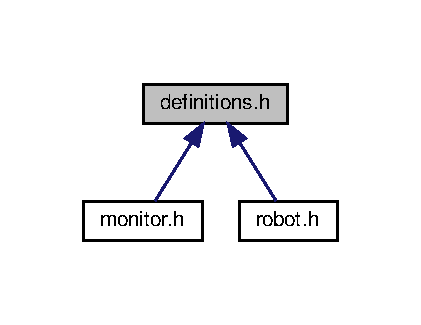
\includegraphics[width=202pt]{definitions_8h__dep__incl}
\end{center}
\end{figure}
\subsection*{Macros}
\begin{DoxyCompactItemize}
\item 
\#define \hyperlink{definitions_8h_aac798eaf6994ddcadd8a38ad8aba234f}{O\+P\+E\+N\+\_\+\+C\+O\+M\+\_\+\+D\+MB}~\textquotesingle{}o\textquotesingle{}
\item 
\#define \hyperlink{definitions_8h_a1b18773c1ce9068c4d38c2cbd2900263}{C\+L\+O\+S\+E\+\_\+\+C\+O\+M\+\_\+\+D\+MB}~\textquotesingle{}C\textquotesingle{}
\item 
\#define \hyperlink{definitions_8h_acf7d51360dcb103fc57604725ec2816d}{D\+M\+B\+\_\+\+P\+I\+NG}~\textquotesingle{}p\textquotesingle{}
\item 
\#define \hyperlink{definitions_8h_a82b279c49221d3cd3d875d521dfb97b9}{D\+M\+B\+\_\+\+I\+D\+LE}~\textquotesingle{}r\textquotesingle{}
\item 
\#define \hyperlink{definitions_8h_a5ebbd37042a6244b4f9d473ae7132780}{D\+M\+B\+\_\+\+S\+T\+A\+R\+T\+\_\+\+W\+I\+T\+H\+O\+U\+T\+\_\+\+WD}~\textquotesingle{}u\textquotesingle{}
\item 
\#define \hyperlink{definitions_8h_adee1628bbc796ba55f4a349895f4e0fa}{D\+M\+B\+\_\+\+S\+T\+A\+R\+T\+\_\+\+W\+I\+T\+H\+\_\+\+WD}~\textquotesingle{}W\textquotesingle{}
\item 
\#define \hyperlink{definitions_8h_a2ca219902014ffb39aab27cca08a948f}{D\+M\+B\+\_\+\+R\+E\+L\+O\+A\+D\+\_\+\+WD}~\textquotesingle{}w\textquotesingle{}
\item 
\#define \hyperlink{definitions_8h_af1737e8fe4da4e8bc2d5db9d26c42462}{D\+M\+B\+\_\+\+G\+E\+T\+\_\+\+V\+B\+AT}~\textquotesingle{}v\textquotesingle{}
\item 
\#define \hyperlink{definitions_8h_ad58c241121e685f26a291aa4bd5f9c80}{D\+M\+B\+\_\+\+I\+S\+\_\+\+B\+U\+SY}~\textquotesingle{}b\textquotesingle{}
\item 
\#define \hyperlink{definitions_8h_ac48dee90eb71d036d001321674abbb8b}{D\+M\+B\+\_\+\+M\+O\+VE}~\textquotesingle{}M\textquotesingle{}
\item 
\#define \hyperlink{definitions_8h_ac6c5492c8100e73f8d30ed36072684db}{D\+M\+B\+\_\+\+T\+U\+RN}~\textquotesingle{}T\textquotesingle{}
\item 
\#define \hyperlink{definitions_8h_ae363a29a4961cd8a646a0ca9199bc6cf}{D\+M\+B\+\_\+\+G\+O\+\_\+\+F\+O\+R\+W\+A\+RD}~\textquotesingle{}F\textquotesingle{}
\item 
\#define \hyperlink{definitions_8h_a499f41cc19a4459de033687049cbbe71}{D\+M\+B\+\_\+\+G\+O\+\_\+\+B\+A\+CK}~\textquotesingle{}B\textquotesingle{}
\item 
\#define \hyperlink{definitions_8h_aefcb838e73a335f1a2a6c914ee2ff752}{D\+M\+B\+\_\+\+G\+O\+\_\+\+L\+E\+FT}~\textquotesingle{}L\textquotesingle{}
\item 
\#define \hyperlink{definitions_8h_ad681962f7b8cf4797ebd48be0405d1b9}{D\+M\+B\+\_\+\+G\+O\+\_\+\+R\+I\+G\+HT}~\textquotesingle{}R\textquotesingle{}
\item 
\#define \hyperlink{definitions_8h_a7308179907a0a2989c162865e7a7979a}{D\+M\+B\+\_\+\+S\+T\+O\+P\+\_\+\+M\+O\+VE}~\textquotesingle{}S\textquotesingle{}
\item 
\#define \hyperlink{definitions_8h_a624686d3af63394ee02f0a197967d44a}{R\+O\+B\+O\+T\+\_\+\+T\+I\+M\+E\+D\+\_\+\+O\+UT}~-\/3
\item 
\#define \hyperlink{definitions_8h_a70a2d5db14b900843364adb7cfe53ac8}{R\+O\+B\+O\+T\+\_\+\+U\+K\+N\+O\+W\+N\+\_\+\+C\+MD}~-\/2
\item 
\#define \hyperlink{definitions_8h_a4aefbbdd5d35999aa0575ab7183148d4}{R\+O\+B\+O\+T\+\_\+\+E\+R\+R\+OR}~-\/1
\item 
\#define \hyperlink{definitions_8h_af1118b8a83d446b4965347bba126a488}{R\+O\+B\+O\+T\+\_\+\+C\+H\+E\+C\+K\+S\+UM}~-\/4
\item 
\#define \hyperlink{definitions_8h_ad7b2f95c0b423fb9784acb897b910c36}{R\+O\+B\+O\+T\+\_\+\+OK}~0
\item 
\#define \hyperlink{definitions_8h_a2a7149bbe097fae8e799ce2ab6f69390}{C\+A\+M\+\_\+\+O\+P\+EN}~\textquotesingle{}A\textquotesingle{}
\item 
\#define \hyperlink{definitions_8h_a675009273c3923e8ad1a6d2818063b61}{C\+A\+M\+\_\+\+C\+L\+O\+SE}~\textquotesingle{}I\textquotesingle{}
\item 
\#define \hyperlink{definitions_8h_a6418778d1f34e618aebd9ca1861ab500}{C\+A\+M\+\_\+\+A\+S\+K\+\_\+\+A\+R\+E\+NA}~\textquotesingle{}y\textquotesingle{}
\item 
\#define \hyperlink{definitions_8h_a15d9063cd3c60755685ceb75df4a7354}{C\+A\+M\+\_\+\+A\+R\+E\+N\+A\+\_\+\+C\+O\+N\+F\+I\+RM}~\textquotesingle{}x\textquotesingle{}
\item 
\#define \hyperlink{definitions_8h_ac836c6abc7e32d2cf7f59ed2a8383ca7}{C\+A\+M\+\_\+\+A\+R\+E\+N\+A\+\_\+\+I\+N\+F\+I\+RM}~\textquotesingle{}z\textquotesingle{}
\item 
\#define \hyperlink{definitions_8h_a74fdb9d00556feb699d3c72bd7b5d5e5}{C\+A\+M\+\_\+\+C\+O\+M\+P\+U\+T\+E\+\_\+\+P\+O\+S\+I\+T\+I\+ON}~\textquotesingle{}p\textquotesingle{}
\item 
\#define \hyperlink{definitions_8h_ae864cfaefbf5a210e67678b2144a289f}{C\+A\+M\+\_\+\+S\+T\+O\+P\+\_\+\+C\+O\+M\+P\+U\+T\+E\+\_\+\+P\+O\+S\+I\+T\+I\+ON}~\textquotesingle{}s\textquotesingle{}
\item 
\#define \hyperlink{definitions_8h_a66c0c4960c1e81c8da8c8e1d4a202352}{D\+M\+B\+\_\+\+B\+A\+T\+\_\+\+L\+OW}~0
\item 
\#define \hyperlink{definitions_8h_aea6ef1c13db1a8a4a29b065d0c3f73e4}{D\+M\+B\+\_\+\+B\+A\+T\+\_\+\+M\+E\+D\+I\+UM}~1
\item 
\#define \hyperlink{definitions_8h_ab34c46794a9de6746a96752668c73754}{D\+M\+B\+\_\+\+B\+A\+T\+\_\+\+H\+I\+GH}~2
\item 
\#define \hyperlink{definitions_8h_a3327443cd321f0c356a5d3d74377892b}{D\+M\+B\+\_\+\+B\+U\+SY}~1
\item 
\#define \hyperlink{definitions_8h_a07650c5f6647c5143bac535fdbeb77d5}{D\+M\+B\+\_\+\+D\+O\+\_\+\+N\+O\+T\+H\+I\+NG}~0
\end{DoxyCompactItemize}


\subsection{Detailed Description}
Various constants used in destjil project. 

\begin{DoxyAuthor}{Author}
P\+E.\+Hladik 
\end{DoxyAuthor}
\begin{DoxyVersion}{Version}
1.\+0 
\end{DoxyVersion}
\begin{DoxyDate}{Date}
06/06/2017 
\end{DoxyDate}


\subsection{Macro Definition Documentation}
\mbox{\Hypertarget{definitions_8h_a15d9063cd3c60755685ceb75df4a7354}\label{definitions_8h_a15d9063cd3c60755685ceb75df4a7354}} 
\index{definitions.\+h@{definitions.\+h}!C\+A\+M\+\_\+\+A\+R\+E\+N\+A\+\_\+\+C\+O\+N\+F\+I\+RM@{C\+A\+M\+\_\+\+A\+R\+E\+N\+A\+\_\+\+C\+O\+N\+F\+I\+RM}}
\index{C\+A\+M\+\_\+\+A\+R\+E\+N\+A\+\_\+\+C\+O\+N\+F\+I\+RM@{C\+A\+M\+\_\+\+A\+R\+E\+N\+A\+\_\+\+C\+O\+N\+F\+I\+RM}!definitions.\+h@{definitions.\+h}}
\subsubsection{\texorpdfstring{C\+A\+M\+\_\+\+A\+R\+E\+N\+A\+\_\+\+C\+O\+N\+F\+I\+RM}{CAM\_ARENA\_CONFIRM}}
{\footnotesize\ttfamily \#define C\+A\+M\+\_\+\+A\+R\+E\+N\+A\+\_\+\+C\+O\+N\+F\+I\+RM~\textquotesingle{}x\textquotesingle{}}



Definition at line 57 of file definitions.\+h.

\mbox{\Hypertarget{definitions_8h_ac836c6abc7e32d2cf7f59ed2a8383ca7}\label{definitions_8h_ac836c6abc7e32d2cf7f59ed2a8383ca7}} 
\index{definitions.\+h@{definitions.\+h}!C\+A\+M\+\_\+\+A\+R\+E\+N\+A\+\_\+\+I\+N\+F\+I\+RM@{C\+A\+M\+\_\+\+A\+R\+E\+N\+A\+\_\+\+I\+N\+F\+I\+RM}}
\index{C\+A\+M\+\_\+\+A\+R\+E\+N\+A\+\_\+\+I\+N\+F\+I\+RM@{C\+A\+M\+\_\+\+A\+R\+E\+N\+A\+\_\+\+I\+N\+F\+I\+RM}!definitions.\+h@{definitions.\+h}}
\subsubsection{\texorpdfstring{C\+A\+M\+\_\+\+A\+R\+E\+N\+A\+\_\+\+I\+N\+F\+I\+RM}{CAM\_ARENA\_INFIRM}}
{\footnotesize\ttfamily \#define C\+A\+M\+\_\+\+A\+R\+E\+N\+A\+\_\+\+I\+N\+F\+I\+RM~\textquotesingle{}z\textquotesingle{}}



Definition at line 58 of file definitions.\+h.

\mbox{\Hypertarget{definitions_8h_a6418778d1f34e618aebd9ca1861ab500}\label{definitions_8h_a6418778d1f34e618aebd9ca1861ab500}} 
\index{definitions.\+h@{definitions.\+h}!C\+A\+M\+\_\+\+A\+S\+K\+\_\+\+A\+R\+E\+NA@{C\+A\+M\+\_\+\+A\+S\+K\+\_\+\+A\+R\+E\+NA}}
\index{C\+A\+M\+\_\+\+A\+S\+K\+\_\+\+A\+R\+E\+NA@{C\+A\+M\+\_\+\+A\+S\+K\+\_\+\+A\+R\+E\+NA}!definitions.\+h@{definitions.\+h}}
\subsubsection{\texorpdfstring{C\+A\+M\+\_\+\+A\+S\+K\+\_\+\+A\+R\+E\+NA}{CAM\_ASK\_ARENA}}
{\footnotesize\ttfamily \#define C\+A\+M\+\_\+\+A\+S\+K\+\_\+\+A\+R\+E\+NA~\textquotesingle{}y\textquotesingle{}}



Definition at line 56 of file definitions.\+h.

\mbox{\Hypertarget{definitions_8h_a675009273c3923e8ad1a6d2818063b61}\label{definitions_8h_a675009273c3923e8ad1a6d2818063b61}} 
\index{definitions.\+h@{definitions.\+h}!C\+A\+M\+\_\+\+C\+L\+O\+SE@{C\+A\+M\+\_\+\+C\+L\+O\+SE}}
\index{C\+A\+M\+\_\+\+C\+L\+O\+SE@{C\+A\+M\+\_\+\+C\+L\+O\+SE}!definitions.\+h@{definitions.\+h}}
\subsubsection{\texorpdfstring{C\+A\+M\+\_\+\+C\+L\+O\+SE}{CAM\_CLOSE}}
{\footnotesize\ttfamily \#define C\+A\+M\+\_\+\+C\+L\+O\+SE~\textquotesingle{}I\textquotesingle{}}



Definition at line 55 of file definitions.\+h.

\mbox{\Hypertarget{definitions_8h_a74fdb9d00556feb699d3c72bd7b5d5e5}\label{definitions_8h_a74fdb9d00556feb699d3c72bd7b5d5e5}} 
\index{definitions.\+h@{definitions.\+h}!C\+A\+M\+\_\+\+C\+O\+M\+P\+U\+T\+E\+\_\+\+P\+O\+S\+I\+T\+I\+ON@{C\+A\+M\+\_\+\+C\+O\+M\+P\+U\+T\+E\+\_\+\+P\+O\+S\+I\+T\+I\+ON}}
\index{C\+A\+M\+\_\+\+C\+O\+M\+P\+U\+T\+E\+\_\+\+P\+O\+S\+I\+T\+I\+ON@{C\+A\+M\+\_\+\+C\+O\+M\+P\+U\+T\+E\+\_\+\+P\+O\+S\+I\+T\+I\+ON}!definitions.\+h@{definitions.\+h}}
\subsubsection{\texorpdfstring{C\+A\+M\+\_\+\+C\+O\+M\+P\+U\+T\+E\+\_\+\+P\+O\+S\+I\+T\+I\+ON}{CAM\_COMPUTE\_POSITION}}
{\footnotesize\ttfamily \#define C\+A\+M\+\_\+\+C\+O\+M\+P\+U\+T\+E\+\_\+\+P\+O\+S\+I\+T\+I\+ON~\textquotesingle{}p\textquotesingle{}}



Definition at line 59 of file definitions.\+h.

\mbox{\Hypertarget{definitions_8h_a2a7149bbe097fae8e799ce2ab6f69390}\label{definitions_8h_a2a7149bbe097fae8e799ce2ab6f69390}} 
\index{definitions.\+h@{definitions.\+h}!C\+A\+M\+\_\+\+O\+P\+EN@{C\+A\+M\+\_\+\+O\+P\+EN}}
\index{C\+A\+M\+\_\+\+O\+P\+EN@{C\+A\+M\+\_\+\+O\+P\+EN}!definitions.\+h@{definitions.\+h}}
\subsubsection{\texorpdfstring{C\+A\+M\+\_\+\+O\+P\+EN}{CAM\_OPEN}}
{\footnotesize\ttfamily \#define C\+A\+M\+\_\+\+O\+P\+EN~\textquotesingle{}A\textquotesingle{}}



Definition at line 54 of file definitions.\+h.

\mbox{\Hypertarget{definitions_8h_ae864cfaefbf5a210e67678b2144a289f}\label{definitions_8h_ae864cfaefbf5a210e67678b2144a289f}} 
\index{definitions.\+h@{definitions.\+h}!C\+A\+M\+\_\+\+S\+T\+O\+P\+\_\+\+C\+O\+M\+P\+U\+T\+E\+\_\+\+P\+O\+S\+I\+T\+I\+ON@{C\+A\+M\+\_\+\+S\+T\+O\+P\+\_\+\+C\+O\+M\+P\+U\+T\+E\+\_\+\+P\+O\+S\+I\+T\+I\+ON}}
\index{C\+A\+M\+\_\+\+S\+T\+O\+P\+\_\+\+C\+O\+M\+P\+U\+T\+E\+\_\+\+P\+O\+S\+I\+T\+I\+ON@{C\+A\+M\+\_\+\+S\+T\+O\+P\+\_\+\+C\+O\+M\+P\+U\+T\+E\+\_\+\+P\+O\+S\+I\+T\+I\+ON}!definitions.\+h@{definitions.\+h}}
\subsubsection{\texorpdfstring{C\+A\+M\+\_\+\+S\+T\+O\+P\+\_\+\+C\+O\+M\+P\+U\+T\+E\+\_\+\+P\+O\+S\+I\+T\+I\+ON}{CAM\_STOP\_COMPUTE\_POSITION}}
{\footnotesize\ttfamily \#define C\+A\+M\+\_\+\+S\+T\+O\+P\+\_\+\+C\+O\+M\+P\+U\+T\+E\+\_\+\+P\+O\+S\+I\+T\+I\+ON~\textquotesingle{}s\textquotesingle{}}



Definition at line 60 of file definitions.\+h.

\mbox{\Hypertarget{definitions_8h_a1b18773c1ce9068c4d38c2cbd2900263}\label{definitions_8h_a1b18773c1ce9068c4d38c2cbd2900263}} 
\index{definitions.\+h@{definitions.\+h}!C\+L\+O\+S\+E\+\_\+\+C\+O\+M\+\_\+\+D\+MB@{C\+L\+O\+S\+E\+\_\+\+C\+O\+M\+\_\+\+D\+MB}}
\index{C\+L\+O\+S\+E\+\_\+\+C\+O\+M\+\_\+\+D\+MB@{C\+L\+O\+S\+E\+\_\+\+C\+O\+M\+\_\+\+D\+MB}!definitions.\+h@{definitions.\+h}}
\subsubsection{\texorpdfstring{C\+L\+O\+S\+E\+\_\+\+C\+O\+M\+\_\+\+D\+MB}{CLOSE\_COM\_DMB}}
{\footnotesize\ttfamily \#define C\+L\+O\+S\+E\+\_\+\+C\+O\+M\+\_\+\+D\+MB~\textquotesingle{}C\textquotesingle{}}



Definition at line 31 of file definitions.\+h.

\mbox{\Hypertarget{definitions_8h_ab34c46794a9de6746a96752668c73754}\label{definitions_8h_ab34c46794a9de6746a96752668c73754}} 
\index{definitions.\+h@{definitions.\+h}!D\+M\+B\+\_\+\+B\+A\+T\+\_\+\+H\+I\+GH@{D\+M\+B\+\_\+\+B\+A\+T\+\_\+\+H\+I\+GH}}
\index{D\+M\+B\+\_\+\+B\+A\+T\+\_\+\+H\+I\+GH@{D\+M\+B\+\_\+\+B\+A\+T\+\_\+\+H\+I\+GH}!definitions.\+h@{definitions.\+h}}
\subsubsection{\texorpdfstring{D\+M\+B\+\_\+\+B\+A\+T\+\_\+\+H\+I\+GH}{DMB\_BAT\_HIGH}}
{\footnotesize\ttfamily \#define D\+M\+B\+\_\+\+B\+A\+T\+\_\+\+H\+I\+GH~2}



Definition at line 64 of file definitions.\+h.

\mbox{\Hypertarget{definitions_8h_a66c0c4960c1e81c8da8c8e1d4a202352}\label{definitions_8h_a66c0c4960c1e81c8da8c8e1d4a202352}} 
\index{definitions.\+h@{definitions.\+h}!D\+M\+B\+\_\+\+B\+A\+T\+\_\+\+L\+OW@{D\+M\+B\+\_\+\+B\+A\+T\+\_\+\+L\+OW}}
\index{D\+M\+B\+\_\+\+B\+A\+T\+\_\+\+L\+OW@{D\+M\+B\+\_\+\+B\+A\+T\+\_\+\+L\+OW}!definitions.\+h@{definitions.\+h}}
\subsubsection{\texorpdfstring{D\+M\+B\+\_\+\+B\+A\+T\+\_\+\+L\+OW}{DMB\_BAT\_LOW}}
{\footnotesize\ttfamily \#define D\+M\+B\+\_\+\+B\+A\+T\+\_\+\+L\+OW~0}



Definition at line 62 of file definitions.\+h.

\mbox{\Hypertarget{definitions_8h_aea6ef1c13db1a8a4a29b065d0c3f73e4}\label{definitions_8h_aea6ef1c13db1a8a4a29b065d0c3f73e4}} 
\index{definitions.\+h@{definitions.\+h}!D\+M\+B\+\_\+\+B\+A\+T\+\_\+\+M\+E\+D\+I\+UM@{D\+M\+B\+\_\+\+B\+A\+T\+\_\+\+M\+E\+D\+I\+UM}}
\index{D\+M\+B\+\_\+\+B\+A\+T\+\_\+\+M\+E\+D\+I\+UM@{D\+M\+B\+\_\+\+B\+A\+T\+\_\+\+M\+E\+D\+I\+UM}!definitions.\+h@{definitions.\+h}}
\subsubsection{\texorpdfstring{D\+M\+B\+\_\+\+B\+A\+T\+\_\+\+M\+E\+D\+I\+UM}{DMB\_BAT\_MEDIUM}}
{\footnotesize\ttfamily \#define D\+M\+B\+\_\+\+B\+A\+T\+\_\+\+M\+E\+D\+I\+UM~1}



Definition at line 63 of file definitions.\+h.

\mbox{\Hypertarget{definitions_8h_a3327443cd321f0c356a5d3d74377892b}\label{definitions_8h_a3327443cd321f0c356a5d3d74377892b}} 
\index{definitions.\+h@{definitions.\+h}!D\+M\+B\+\_\+\+B\+U\+SY@{D\+M\+B\+\_\+\+B\+U\+SY}}
\index{D\+M\+B\+\_\+\+B\+U\+SY@{D\+M\+B\+\_\+\+B\+U\+SY}!definitions.\+h@{definitions.\+h}}
\subsubsection{\texorpdfstring{D\+M\+B\+\_\+\+B\+U\+SY}{DMB\_BUSY}}
{\footnotesize\ttfamily \#define D\+M\+B\+\_\+\+B\+U\+SY~1}



Definition at line 66 of file definitions.\+h.

\mbox{\Hypertarget{definitions_8h_a07650c5f6647c5143bac535fdbeb77d5}\label{definitions_8h_a07650c5f6647c5143bac535fdbeb77d5}} 
\index{definitions.\+h@{definitions.\+h}!D\+M\+B\+\_\+\+D\+O\+\_\+\+N\+O\+T\+H\+I\+NG@{D\+M\+B\+\_\+\+D\+O\+\_\+\+N\+O\+T\+H\+I\+NG}}
\index{D\+M\+B\+\_\+\+D\+O\+\_\+\+N\+O\+T\+H\+I\+NG@{D\+M\+B\+\_\+\+D\+O\+\_\+\+N\+O\+T\+H\+I\+NG}!definitions.\+h@{definitions.\+h}}
\subsubsection{\texorpdfstring{D\+M\+B\+\_\+\+D\+O\+\_\+\+N\+O\+T\+H\+I\+NG}{DMB\_DO\_NOTHING}}
{\footnotesize\ttfamily \#define D\+M\+B\+\_\+\+D\+O\+\_\+\+N\+O\+T\+H\+I\+NG~0}



Definition at line 67 of file definitions.\+h.

\mbox{\Hypertarget{definitions_8h_af1737e8fe4da4e8bc2d5db9d26c42462}\label{definitions_8h_af1737e8fe4da4e8bc2d5db9d26c42462}} 
\index{definitions.\+h@{definitions.\+h}!D\+M\+B\+\_\+\+G\+E\+T\+\_\+\+V\+B\+AT@{D\+M\+B\+\_\+\+G\+E\+T\+\_\+\+V\+B\+AT}}
\index{D\+M\+B\+\_\+\+G\+E\+T\+\_\+\+V\+B\+AT@{D\+M\+B\+\_\+\+G\+E\+T\+\_\+\+V\+B\+AT}!definitions.\+h@{definitions.\+h}}
\subsubsection{\texorpdfstring{D\+M\+B\+\_\+\+G\+E\+T\+\_\+\+V\+B\+AT}{DMB\_GET\_VBAT}}
{\footnotesize\ttfamily \#define D\+M\+B\+\_\+\+G\+E\+T\+\_\+\+V\+B\+AT~\textquotesingle{}v\textquotesingle{}}



Definition at line 38 of file definitions.\+h.

\mbox{\Hypertarget{definitions_8h_a499f41cc19a4459de033687049cbbe71}\label{definitions_8h_a499f41cc19a4459de033687049cbbe71}} 
\index{definitions.\+h@{definitions.\+h}!D\+M\+B\+\_\+\+G\+O\+\_\+\+B\+A\+CK@{D\+M\+B\+\_\+\+G\+O\+\_\+\+B\+A\+CK}}
\index{D\+M\+B\+\_\+\+G\+O\+\_\+\+B\+A\+CK@{D\+M\+B\+\_\+\+G\+O\+\_\+\+B\+A\+CK}!definitions.\+h@{definitions.\+h}}
\subsubsection{\texorpdfstring{D\+M\+B\+\_\+\+G\+O\+\_\+\+B\+A\+CK}{DMB\_GO\_BACK}}
{\footnotesize\ttfamily \#define D\+M\+B\+\_\+\+G\+O\+\_\+\+B\+A\+CK~\textquotesingle{}B\textquotesingle{}}



Definition at line 43 of file definitions.\+h.

\mbox{\Hypertarget{definitions_8h_ae363a29a4961cd8a646a0ca9199bc6cf}\label{definitions_8h_ae363a29a4961cd8a646a0ca9199bc6cf}} 
\index{definitions.\+h@{definitions.\+h}!D\+M\+B\+\_\+\+G\+O\+\_\+\+F\+O\+R\+W\+A\+RD@{D\+M\+B\+\_\+\+G\+O\+\_\+\+F\+O\+R\+W\+A\+RD}}
\index{D\+M\+B\+\_\+\+G\+O\+\_\+\+F\+O\+R\+W\+A\+RD@{D\+M\+B\+\_\+\+G\+O\+\_\+\+F\+O\+R\+W\+A\+RD}!definitions.\+h@{definitions.\+h}}
\subsubsection{\texorpdfstring{D\+M\+B\+\_\+\+G\+O\+\_\+\+F\+O\+R\+W\+A\+RD}{DMB\_GO\_FORWARD}}
{\footnotesize\ttfamily \#define D\+M\+B\+\_\+\+G\+O\+\_\+\+F\+O\+R\+W\+A\+RD~\textquotesingle{}F\textquotesingle{}}



Definition at line 42 of file definitions.\+h.

\mbox{\Hypertarget{definitions_8h_aefcb838e73a335f1a2a6c914ee2ff752}\label{definitions_8h_aefcb838e73a335f1a2a6c914ee2ff752}} 
\index{definitions.\+h@{definitions.\+h}!D\+M\+B\+\_\+\+G\+O\+\_\+\+L\+E\+FT@{D\+M\+B\+\_\+\+G\+O\+\_\+\+L\+E\+FT}}
\index{D\+M\+B\+\_\+\+G\+O\+\_\+\+L\+E\+FT@{D\+M\+B\+\_\+\+G\+O\+\_\+\+L\+E\+FT}!definitions.\+h@{definitions.\+h}}
\subsubsection{\texorpdfstring{D\+M\+B\+\_\+\+G\+O\+\_\+\+L\+E\+FT}{DMB\_GO\_LEFT}}
{\footnotesize\ttfamily \#define D\+M\+B\+\_\+\+G\+O\+\_\+\+L\+E\+FT~\textquotesingle{}L\textquotesingle{}}



Definition at line 44 of file definitions.\+h.

\mbox{\Hypertarget{definitions_8h_ad681962f7b8cf4797ebd48be0405d1b9}\label{definitions_8h_ad681962f7b8cf4797ebd48be0405d1b9}} 
\index{definitions.\+h@{definitions.\+h}!D\+M\+B\+\_\+\+G\+O\+\_\+\+R\+I\+G\+HT@{D\+M\+B\+\_\+\+G\+O\+\_\+\+R\+I\+G\+HT}}
\index{D\+M\+B\+\_\+\+G\+O\+\_\+\+R\+I\+G\+HT@{D\+M\+B\+\_\+\+G\+O\+\_\+\+R\+I\+G\+HT}!definitions.\+h@{definitions.\+h}}
\subsubsection{\texorpdfstring{D\+M\+B\+\_\+\+G\+O\+\_\+\+R\+I\+G\+HT}{DMB\_GO\_RIGHT}}
{\footnotesize\ttfamily \#define D\+M\+B\+\_\+\+G\+O\+\_\+\+R\+I\+G\+HT~\textquotesingle{}R\textquotesingle{}}



Definition at line 45 of file definitions.\+h.

\mbox{\Hypertarget{definitions_8h_a82b279c49221d3cd3d875d521dfb97b9}\label{definitions_8h_a82b279c49221d3cd3d875d521dfb97b9}} 
\index{definitions.\+h@{definitions.\+h}!D\+M\+B\+\_\+\+I\+D\+LE@{D\+M\+B\+\_\+\+I\+D\+LE}}
\index{D\+M\+B\+\_\+\+I\+D\+LE@{D\+M\+B\+\_\+\+I\+D\+LE}!definitions.\+h@{definitions.\+h}}
\subsubsection{\texorpdfstring{D\+M\+B\+\_\+\+I\+D\+LE}{DMB\_IDLE}}
{\footnotesize\ttfamily \#define D\+M\+B\+\_\+\+I\+D\+LE~\textquotesingle{}r\textquotesingle{}}



Definition at line 34 of file definitions.\+h.

\mbox{\Hypertarget{definitions_8h_ad58c241121e685f26a291aa4bd5f9c80}\label{definitions_8h_ad58c241121e685f26a291aa4bd5f9c80}} 
\index{definitions.\+h@{definitions.\+h}!D\+M\+B\+\_\+\+I\+S\+\_\+\+B\+U\+SY@{D\+M\+B\+\_\+\+I\+S\+\_\+\+B\+U\+SY}}
\index{D\+M\+B\+\_\+\+I\+S\+\_\+\+B\+U\+SY@{D\+M\+B\+\_\+\+I\+S\+\_\+\+B\+U\+SY}!definitions.\+h@{definitions.\+h}}
\subsubsection{\texorpdfstring{D\+M\+B\+\_\+\+I\+S\+\_\+\+B\+U\+SY}{DMB\_IS\_BUSY}}
{\footnotesize\ttfamily \#define D\+M\+B\+\_\+\+I\+S\+\_\+\+B\+U\+SY~\textquotesingle{}b\textquotesingle{}}



Definition at line 39 of file definitions.\+h.

\mbox{\Hypertarget{definitions_8h_ac48dee90eb71d036d001321674abbb8b}\label{definitions_8h_ac48dee90eb71d036d001321674abbb8b}} 
\index{definitions.\+h@{definitions.\+h}!D\+M\+B\+\_\+\+M\+O\+VE@{D\+M\+B\+\_\+\+M\+O\+VE}}
\index{D\+M\+B\+\_\+\+M\+O\+VE@{D\+M\+B\+\_\+\+M\+O\+VE}!definitions.\+h@{definitions.\+h}}
\subsubsection{\texorpdfstring{D\+M\+B\+\_\+\+M\+O\+VE}{DMB\_MOVE}}
{\footnotesize\ttfamily \#define D\+M\+B\+\_\+\+M\+O\+VE~\textquotesingle{}M\textquotesingle{}}



Definition at line 40 of file definitions.\+h.

\mbox{\Hypertarget{definitions_8h_acf7d51360dcb103fc57604725ec2816d}\label{definitions_8h_acf7d51360dcb103fc57604725ec2816d}} 
\index{definitions.\+h@{definitions.\+h}!D\+M\+B\+\_\+\+P\+I\+NG@{D\+M\+B\+\_\+\+P\+I\+NG}}
\index{D\+M\+B\+\_\+\+P\+I\+NG@{D\+M\+B\+\_\+\+P\+I\+NG}!definitions.\+h@{definitions.\+h}}
\subsubsection{\texorpdfstring{D\+M\+B\+\_\+\+P\+I\+NG}{DMB\_PING}}
{\footnotesize\ttfamily \#define D\+M\+B\+\_\+\+P\+I\+NG~\textquotesingle{}p\textquotesingle{}}



Definition at line 33 of file definitions.\+h.

\mbox{\Hypertarget{definitions_8h_a2ca219902014ffb39aab27cca08a948f}\label{definitions_8h_a2ca219902014ffb39aab27cca08a948f}} 
\index{definitions.\+h@{definitions.\+h}!D\+M\+B\+\_\+\+R\+E\+L\+O\+A\+D\+\_\+\+WD@{D\+M\+B\+\_\+\+R\+E\+L\+O\+A\+D\+\_\+\+WD}}
\index{D\+M\+B\+\_\+\+R\+E\+L\+O\+A\+D\+\_\+\+WD@{D\+M\+B\+\_\+\+R\+E\+L\+O\+A\+D\+\_\+\+WD}!definitions.\+h@{definitions.\+h}}
\subsubsection{\texorpdfstring{D\+M\+B\+\_\+\+R\+E\+L\+O\+A\+D\+\_\+\+WD}{DMB\_RELOAD\_WD}}
{\footnotesize\ttfamily \#define D\+M\+B\+\_\+\+R\+E\+L\+O\+A\+D\+\_\+\+WD~\textquotesingle{}w\textquotesingle{}}



Definition at line 37 of file definitions.\+h.

\mbox{\Hypertarget{definitions_8h_adee1628bbc796ba55f4a349895f4e0fa}\label{definitions_8h_adee1628bbc796ba55f4a349895f4e0fa}} 
\index{definitions.\+h@{definitions.\+h}!D\+M\+B\+\_\+\+S\+T\+A\+R\+T\+\_\+\+W\+I\+T\+H\+\_\+\+WD@{D\+M\+B\+\_\+\+S\+T\+A\+R\+T\+\_\+\+W\+I\+T\+H\+\_\+\+WD}}
\index{D\+M\+B\+\_\+\+S\+T\+A\+R\+T\+\_\+\+W\+I\+T\+H\+\_\+\+WD@{D\+M\+B\+\_\+\+S\+T\+A\+R\+T\+\_\+\+W\+I\+T\+H\+\_\+\+WD}!definitions.\+h@{definitions.\+h}}
\subsubsection{\texorpdfstring{D\+M\+B\+\_\+\+S\+T\+A\+R\+T\+\_\+\+W\+I\+T\+H\+\_\+\+WD}{DMB\_START\_WITH\_WD}}
{\footnotesize\ttfamily \#define D\+M\+B\+\_\+\+S\+T\+A\+R\+T\+\_\+\+W\+I\+T\+H\+\_\+\+WD~\textquotesingle{}W\textquotesingle{}}



Definition at line 36 of file definitions.\+h.

\mbox{\Hypertarget{definitions_8h_a5ebbd37042a6244b4f9d473ae7132780}\label{definitions_8h_a5ebbd37042a6244b4f9d473ae7132780}} 
\index{definitions.\+h@{definitions.\+h}!D\+M\+B\+\_\+\+S\+T\+A\+R\+T\+\_\+\+W\+I\+T\+H\+O\+U\+T\+\_\+\+WD@{D\+M\+B\+\_\+\+S\+T\+A\+R\+T\+\_\+\+W\+I\+T\+H\+O\+U\+T\+\_\+\+WD}}
\index{D\+M\+B\+\_\+\+S\+T\+A\+R\+T\+\_\+\+W\+I\+T\+H\+O\+U\+T\+\_\+\+WD@{D\+M\+B\+\_\+\+S\+T\+A\+R\+T\+\_\+\+W\+I\+T\+H\+O\+U\+T\+\_\+\+WD}!definitions.\+h@{definitions.\+h}}
\subsubsection{\texorpdfstring{D\+M\+B\+\_\+\+S\+T\+A\+R\+T\+\_\+\+W\+I\+T\+H\+O\+U\+T\+\_\+\+WD}{DMB\_START\_WITHOUT\_WD}}
{\footnotesize\ttfamily \#define D\+M\+B\+\_\+\+S\+T\+A\+R\+T\+\_\+\+W\+I\+T\+H\+O\+U\+T\+\_\+\+WD~\textquotesingle{}u\textquotesingle{}}



Definition at line 35 of file definitions.\+h.

\mbox{\Hypertarget{definitions_8h_a7308179907a0a2989c162865e7a7979a}\label{definitions_8h_a7308179907a0a2989c162865e7a7979a}} 
\index{definitions.\+h@{definitions.\+h}!D\+M\+B\+\_\+\+S\+T\+O\+P\+\_\+\+M\+O\+VE@{D\+M\+B\+\_\+\+S\+T\+O\+P\+\_\+\+M\+O\+VE}}
\index{D\+M\+B\+\_\+\+S\+T\+O\+P\+\_\+\+M\+O\+VE@{D\+M\+B\+\_\+\+S\+T\+O\+P\+\_\+\+M\+O\+VE}!definitions.\+h@{definitions.\+h}}
\subsubsection{\texorpdfstring{D\+M\+B\+\_\+\+S\+T\+O\+P\+\_\+\+M\+O\+VE}{DMB\_STOP\_MOVE}}
{\footnotesize\ttfamily \#define D\+M\+B\+\_\+\+S\+T\+O\+P\+\_\+\+M\+O\+VE~\textquotesingle{}S\textquotesingle{}}



Definition at line 46 of file definitions.\+h.

\mbox{\Hypertarget{definitions_8h_ac6c5492c8100e73f8d30ed36072684db}\label{definitions_8h_ac6c5492c8100e73f8d30ed36072684db}} 
\index{definitions.\+h@{definitions.\+h}!D\+M\+B\+\_\+\+T\+U\+RN@{D\+M\+B\+\_\+\+T\+U\+RN}}
\index{D\+M\+B\+\_\+\+T\+U\+RN@{D\+M\+B\+\_\+\+T\+U\+RN}!definitions.\+h@{definitions.\+h}}
\subsubsection{\texorpdfstring{D\+M\+B\+\_\+\+T\+U\+RN}{DMB\_TURN}}
{\footnotesize\ttfamily \#define D\+M\+B\+\_\+\+T\+U\+RN~\textquotesingle{}T\textquotesingle{}}



Definition at line 41 of file definitions.\+h.

\mbox{\Hypertarget{definitions_8h_aac798eaf6994ddcadd8a38ad8aba234f}\label{definitions_8h_aac798eaf6994ddcadd8a38ad8aba234f}} 
\index{definitions.\+h@{definitions.\+h}!O\+P\+E\+N\+\_\+\+C\+O\+M\+\_\+\+D\+MB@{O\+P\+E\+N\+\_\+\+C\+O\+M\+\_\+\+D\+MB}}
\index{O\+P\+E\+N\+\_\+\+C\+O\+M\+\_\+\+D\+MB@{O\+P\+E\+N\+\_\+\+C\+O\+M\+\_\+\+D\+MB}!definitions.\+h@{definitions.\+h}}
\subsubsection{\texorpdfstring{O\+P\+E\+N\+\_\+\+C\+O\+M\+\_\+\+D\+MB}{OPEN\_COM\_DMB}}
{\footnotesize\ttfamily \#define O\+P\+E\+N\+\_\+\+C\+O\+M\+\_\+\+D\+MB~\textquotesingle{}o\textquotesingle{}}



Definition at line 30 of file definitions.\+h.

\mbox{\Hypertarget{definitions_8h_af1118b8a83d446b4965347bba126a488}\label{definitions_8h_af1118b8a83d446b4965347bba126a488}} 
\index{definitions.\+h@{definitions.\+h}!R\+O\+B\+O\+T\+\_\+\+C\+H\+E\+C\+K\+S\+UM@{R\+O\+B\+O\+T\+\_\+\+C\+H\+E\+C\+K\+S\+UM}}
\index{R\+O\+B\+O\+T\+\_\+\+C\+H\+E\+C\+K\+S\+UM@{R\+O\+B\+O\+T\+\_\+\+C\+H\+E\+C\+K\+S\+UM}!definitions.\+h@{definitions.\+h}}
\subsubsection{\texorpdfstring{R\+O\+B\+O\+T\+\_\+\+C\+H\+E\+C\+K\+S\+UM}{ROBOT\_CHECKSUM}}
{\footnotesize\ttfamily \#define R\+O\+B\+O\+T\+\_\+\+C\+H\+E\+C\+K\+S\+UM~-\/4}



Definition at line 51 of file definitions.\+h.

\mbox{\Hypertarget{definitions_8h_a4aefbbdd5d35999aa0575ab7183148d4}\label{definitions_8h_a4aefbbdd5d35999aa0575ab7183148d4}} 
\index{definitions.\+h@{definitions.\+h}!R\+O\+B\+O\+T\+\_\+\+E\+R\+R\+OR@{R\+O\+B\+O\+T\+\_\+\+E\+R\+R\+OR}}
\index{R\+O\+B\+O\+T\+\_\+\+E\+R\+R\+OR@{R\+O\+B\+O\+T\+\_\+\+E\+R\+R\+OR}!definitions.\+h@{definitions.\+h}}
\subsubsection{\texorpdfstring{R\+O\+B\+O\+T\+\_\+\+E\+R\+R\+OR}{ROBOT\_ERROR}}
{\footnotesize\ttfamily \#define R\+O\+B\+O\+T\+\_\+\+E\+R\+R\+OR~-\/1}



Definition at line 50 of file definitions.\+h.

\mbox{\Hypertarget{definitions_8h_ad7b2f95c0b423fb9784acb897b910c36}\label{definitions_8h_ad7b2f95c0b423fb9784acb897b910c36}} 
\index{definitions.\+h@{definitions.\+h}!R\+O\+B\+O\+T\+\_\+\+OK@{R\+O\+B\+O\+T\+\_\+\+OK}}
\index{R\+O\+B\+O\+T\+\_\+\+OK@{R\+O\+B\+O\+T\+\_\+\+OK}!definitions.\+h@{definitions.\+h}}
\subsubsection{\texorpdfstring{R\+O\+B\+O\+T\+\_\+\+OK}{ROBOT\_OK}}
{\footnotesize\ttfamily \#define R\+O\+B\+O\+T\+\_\+\+OK~0}



Definition at line 52 of file definitions.\+h.

\mbox{\Hypertarget{definitions_8h_a624686d3af63394ee02f0a197967d44a}\label{definitions_8h_a624686d3af63394ee02f0a197967d44a}} 
\index{definitions.\+h@{definitions.\+h}!R\+O\+B\+O\+T\+\_\+\+T\+I\+M\+E\+D\+\_\+\+O\+UT@{R\+O\+B\+O\+T\+\_\+\+T\+I\+M\+E\+D\+\_\+\+O\+UT}}
\index{R\+O\+B\+O\+T\+\_\+\+T\+I\+M\+E\+D\+\_\+\+O\+UT@{R\+O\+B\+O\+T\+\_\+\+T\+I\+M\+E\+D\+\_\+\+O\+UT}!definitions.\+h@{definitions.\+h}}
\subsubsection{\texorpdfstring{R\+O\+B\+O\+T\+\_\+\+T\+I\+M\+E\+D\+\_\+\+O\+UT}{ROBOT\_TIMED\_OUT}}
{\footnotesize\ttfamily \#define R\+O\+B\+O\+T\+\_\+\+T\+I\+M\+E\+D\+\_\+\+O\+UT~-\/3}



Definition at line 48 of file definitions.\+h.

\mbox{\Hypertarget{definitions_8h_a70a2d5db14b900843364adb7cfe53ac8}\label{definitions_8h_a70a2d5db14b900843364adb7cfe53ac8}} 
\index{definitions.\+h@{definitions.\+h}!R\+O\+B\+O\+T\+\_\+\+U\+K\+N\+O\+W\+N\+\_\+\+C\+MD@{R\+O\+B\+O\+T\+\_\+\+U\+K\+N\+O\+W\+N\+\_\+\+C\+MD}}
\index{R\+O\+B\+O\+T\+\_\+\+U\+K\+N\+O\+W\+N\+\_\+\+C\+MD@{R\+O\+B\+O\+T\+\_\+\+U\+K\+N\+O\+W\+N\+\_\+\+C\+MD}!definitions.\+h@{definitions.\+h}}
\subsubsection{\texorpdfstring{R\+O\+B\+O\+T\+\_\+\+U\+K\+N\+O\+W\+N\+\_\+\+C\+MD}{ROBOT\_UKNOWN\_CMD}}
{\footnotesize\ttfamily \#define R\+O\+B\+O\+T\+\_\+\+U\+K\+N\+O\+W\+N\+\_\+\+C\+MD~-\/2}



Definition at line 49 of file definitions.\+h.


\hypertarget{image_8h}{}\section{image.\+h File Reference}
\label{image_8h}\index{image.\+h@{image.\+h}}


Functions for image treatment.  


{\ttfamily \#include $<$raspicam/raspicam\+\_\+cv.\+h$>$}\newline
{\ttfamily \#include \char`\"{}opencv2/imgproc/imgproc.\+hpp\char`\"{}}\newline
{\ttfamily \#include $<$unistd.\+h$>$}\newline
{\ttfamily \#include $<$math.\+h$>$}\newline
Include dependency graph for image.\+h\+:\nopagebreak
\begin{figure}[H]
\begin{center}
\leavevmode
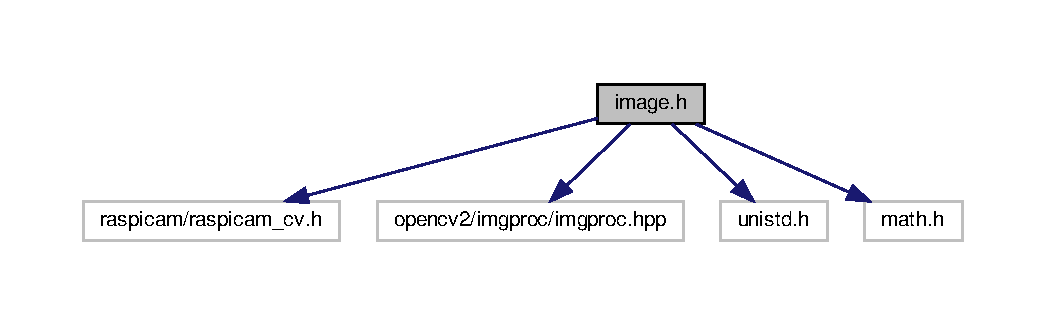
\includegraphics[width=350pt]{image_8h__incl}
\end{center}
\end{figure}
This graph shows which files directly or indirectly include this file\+:\nopagebreak
\begin{figure}[H]
\begin{center}
\leavevmode
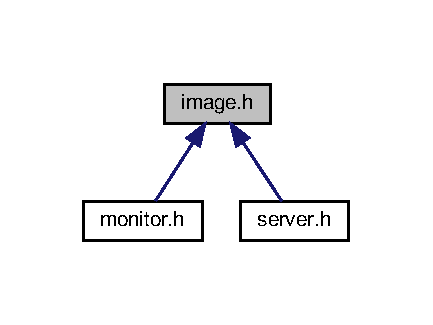
\includegraphics[width=208pt]{image_8h__dep__incl}
\end{center}
\end{figure}
\subsection*{Classes}
\begin{DoxyCompactItemize}
\item 
struct \hyperlink{struct_position}{Position}
\end{DoxyCompactItemize}
\subsection*{Macros}
\begin{DoxyCompactItemize}
\item 
\#define \hyperlink{image_8h_a241aeeb764887ae5e3de58b98f04b16d}{W\+I\+D\+TH}~480
\item 
\#define \hyperlink{image_8h_aed89bd71aee8be823e8a20ec4e093c1e}{H\+E\+I\+G\+HT}~360
\end{DoxyCompactItemize}
\subsection*{Typedefs}
\begin{DoxyCompactItemize}
\item 
typedef Mat \hyperlink{image_8h_a466446fef9c0348568bc6743186d1a38}{Image}
\item 
typedef Raspi\+Cam\+\_\+\+Cv \hyperlink{image_8h_a739dda3f6f6ddbab22617837b43a692a}{Camera}
\item 
typedef Rect \hyperlink{image_8h_aa856a7cb8a1535c9f13096bede6c8586}{Arene}
\item 
typedef vector$<$ unsigned char $>$ \hyperlink{image_8h_a9ac2855e21920c676a108df386ff9415}{Jpg}
\end{DoxyCompactItemize}
\subsection*{Functions}
\begin{DoxyCompactItemize}
\item 
int \hyperlink{image_8h_aca0662ab31eac7fdb2d64fecc52ff1da}{open\+\_\+camera} (\hyperlink{image_8h_a739dda3f6f6ddbab22617837b43a692a}{Camera} $\ast$camera)
\begin{DoxyCompactList}\small\item\em Ouvre une camera. \end{DoxyCompactList}\item 
void \hyperlink{image_8h_a19eac11a04cb4b86fd32e6a36445ad5d}{close\+\_\+camera} (\hyperlink{image_8h_a739dda3f6f6ddbab22617837b43a692a}{Camera} $\ast$camera)
\begin{DoxyCompactList}\small\item\em Ferme la camera passé en paramètre. \end{DoxyCompactList}\item 
void \hyperlink{image_8h_ad904f3348c2d44f9c82435c94cd83844}{get\+\_\+image} (\hyperlink{image_8h_a739dda3f6f6ddbab22617837b43a692a}{Camera} $\ast$camera, \hyperlink{image_8h_a466446fef9c0348568bc6743186d1a38}{Image} $\ast$mon\+Image, const char $\ast$fichier=N\+U\+LL)
\begin{DoxyCompactList}\small\item\em Capture une image avec la camera passée en entrée. En cas de test sans camera, la fonction charge une image. \end{DoxyCompactList}\item 
int \hyperlink{image_8h_acad45df4061a55f17be0db97c1406249}{detect\+\_\+arena} (\hyperlink{image_8h_a466446fef9c0348568bc6743186d1a38}{Image} $\ast$mon\+Image, \hyperlink{image_8h_aa856a7cb8a1535c9f13096bede6c8586}{Arene} $\ast$rectangle)
\begin{DoxyCompactList}\small\item\em Détecte une arène dans une image fournis en paramètre. \end{DoxyCompactList}\item 
void \hyperlink{image_8h_a5ffd032a466af45a505fb46252194bbf}{draw\+\_\+arena} (\hyperlink{image_8h_a466446fef9c0348568bc6743186d1a38}{Image} $\ast$img\+Input, \hyperlink{image_8h_a466446fef9c0348568bc6743186d1a38}{Image} $\ast$img\+Output, \hyperlink{image_8h_aa856a7cb8a1535c9f13096bede6c8586}{Arene} $\ast$mon\+Arene)
\begin{DoxyCompactList}\small\item\em Dessine le plus petit rectangle contenant l\textquotesingle{}arène. \end{DoxyCompactList}\item 
int \hyperlink{image_8h_af9f6e2dd4409486f2f6446d1a8a02c40}{detect\+\_\+position} (\hyperlink{image_8h_a466446fef9c0348568bc6743186d1a38}{Image} $\ast$img\+Input, \hyperlink{struct_position}{Position} $\ast$pos\+Triangle, \hyperlink{image_8h_aa856a7cb8a1535c9f13096bede6c8586}{Arene} $\ast$mon\+Arene=N\+U\+LL)
\begin{DoxyCompactList}\small\item\em Détecte la position d\textquotesingle{}un robot. \end{DoxyCompactList}\item 
void \hyperlink{image_8h_a869c3946d4a414b8730ca4f91fbd9556}{draw\+\_\+position} (\hyperlink{image_8h_a466446fef9c0348568bc6743186d1a38}{Image} $\ast$img\+Input, \hyperlink{image_8h_a466446fef9c0348568bc6743186d1a38}{Image} $\ast$img\+Output, \hyperlink{struct_position}{Position} $\ast$position\+Robot)
\begin{DoxyCompactList}\small\item\em Dessine sur une image en entrée la position d\textquotesingle{}un robot et sa direction. \end{DoxyCompactList}\item 
void \hyperlink{image_8h_a909ca7577f0ac2e4bd0ea21291690dce}{compress\+\_\+image} (\hyperlink{image_8h_a466446fef9c0348568bc6743186d1a38}{Image} $\ast$img\+Input, \hyperlink{image_8h_a9ac2855e21920c676a108df386ff9415}{Jpg} $\ast$image\+Compress)
\begin{DoxyCompactList}\small\item\em Détecte la position d\textquotesingle{}un robot. \end{DoxyCompactList}\end{DoxyCompactItemize}


\subsection{Detailed Description}
Functions for image treatment. 

\begin{DoxyAuthor}{Author}
L.\+Senaneuch 
\end{DoxyAuthor}
\begin{DoxyVersion}{Version}
1.\+0 
\end{DoxyVersion}
\begin{DoxyDate}{Date}
06/06/2017
\end{DoxyDate}
This file use open\+C\+V2 library for picture processing. This allow to detect arena and robot. 

\subsection{Macro Definition Documentation}
\mbox{\Hypertarget{image_8h_aed89bd71aee8be823e8a20ec4e093c1e}\label{image_8h_aed89bd71aee8be823e8a20ec4e093c1e}} 
\index{image.\+h@{image.\+h}!H\+E\+I\+G\+HT@{H\+E\+I\+G\+HT}}
\index{H\+E\+I\+G\+HT@{H\+E\+I\+G\+HT}!image.\+h@{image.\+h}}
\subsubsection{\texorpdfstring{H\+E\+I\+G\+HT}{HEIGHT}}
{\footnotesize\ttfamily \#define H\+E\+I\+G\+HT~360}



Definition at line 45 of file image.\+h.

\mbox{\Hypertarget{image_8h_a241aeeb764887ae5e3de58b98f04b16d}\label{image_8h_a241aeeb764887ae5e3de58b98f04b16d}} 
\index{image.\+h@{image.\+h}!W\+I\+D\+TH@{W\+I\+D\+TH}}
\index{W\+I\+D\+TH@{W\+I\+D\+TH}!image.\+h@{image.\+h}}
\subsubsection{\texorpdfstring{W\+I\+D\+TH}{WIDTH}}
{\footnotesize\ttfamily \#define W\+I\+D\+TH~480}



Definition at line 44 of file image.\+h.



\subsection{Typedef Documentation}
\mbox{\Hypertarget{image_8h_aa856a7cb8a1535c9f13096bede6c8586}\label{image_8h_aa856a7cb8a1535c9f13096bede6c8586}} 
\index{image.\+h@{image.\+h}!Arene@{Arene}}
\index{Arene@{Arene}!image.\+h@{image.\+h}}
\subsubsection{\texorpdfstring{Arene}{Arene}}
{\footnotesize\ttfamily typedef Rect \hyperlink{image_8h_aa856a7cb8a1535c9f13096bede6c8586}{Arene}}



Definition at line 66 of file image.\+h.

\mbox{\Hypertarget{image_8h_a739dda3f6f6ddbab22617837b43a692a}\label{image_8h_a739dda3f6f6ddbab22617837b43a692a}} 
\index{image.\+h@{image.\+h}!Camera@{Camera}}
\index{Camera@{Camera}!image.\+h@{image.\+h}}
\subsubsection{\texorpdfstring{Camera}{Camera}}
{\footnotesize\ttfamily typedef Raspi\+Cam\+\_\+\+Cv \hyperlink{image_8h_a739dda3f6f6ddbab22617837b43a692a}{Camera}}



Definition at line 58 of file image.\+h.

\mbox{\Hypertarget{image_8h_a466446fef9c0348568bc6743186d1a38}\label{image_8h_a466446fef9c0348568bc6743186d1a38}} 
\index{image.\+h@{image.\+h}!Image@{Image}}
\index{Image@{Image}!image.\+h@{image.\+h}}
\subsubsection{\texorpdfstring{Image}{Image}}
{\footnotesize\ttfamily typedef Mat \hyperlink{image_8h_a466446fef9c0348568bc6743186d1a38}{Image}}



Definition at line 55 of file image.\+h.

\mbox{\Hypertarget{image_8h_a9ac2855e21920c676a108df386ff9415}\label{image_8h_a9ac2855e21920c676a108df386ff9415}} 
\index{image.\+h@{image.\+h}!Jpg@{Jpg}}
\index{Jpg@{Jpg}!image.\+h@{image.\+h}}
\subsubsection{\texorpdfstring{Jpg}{Jpg}}
{\footnotesize\ttfamily typedef vector$<$unsigned char$>$ \hyperlink{image_8h_a9ac2855e21920c676a108df386ff9415}{Jpg}}



Definition at line 67 of file image.\+h.



\subsection{Function Documentation}
\mbox{\Hypertarget{image_8h_a19eac11a04cb4b86fd32e6a36445ad5d}\label{image_8h_a19eac11a04cb4b86fd32e6a36445ad5d}} 
\index{image.\+h@{image.\+h}!close\+\_\+camera@{close\+\_\+camera}}
\index{close\+\_\+camera@{close\+\_\+camera}!image.\+h@{image.\+h}}
\subsubsection{\texorpdfstring{close\+\_\+camera()}{close\_camera()}}
{\footnotesize\ttfamily void close\+\_\+camera (\begin{DoxyParamCaption}\item[{\hyperlink{image_8h_a739dda3f6f6ddbab22617837b43a692a}{Camera} $\ast$}]{camera }\end{DoxyParamCaption})}



Ferme la camera passé en paramètre. 


\begin{DoxyParams}{Parameters}
{\em camera} & Pointeur sur la camera à fermer \\
\hline
\end{DoxyParams}
\mbox{\Hypertarget{image_8h_a909ca7577f0ac2e4bd0ea21291690dce}\label{image_8h_a909ca7577f0ac2e4bd0ea21291690dce}} 
\index{image.\+h@{image.\+h}!compress\+\_\+image@{compress\+\_\+image}}
\index{compress\+\_\+image@{compress\+\_\+image}!image.\+h@{image.\+h}}
\subsubsection{\texorpdfstring{compress\+\_\+image()}{compress\_image()}}
{\footnotesize\ttfamily void compress\+\_\+image (\begin{DoxyParamCaption}\item[{\hyperlink{image_8h_a466446fef9c0348568bc6743186d1a38}{Image} $\ast$}]{img\+Input,  }\item[{\hyperlink{image_8h_a9ac2855e21920c676a108df386ff9415}{Jpg} $\ast$}]{image\+Compress }\end{DoxyParamCaption})}



Détecte la position d\textquotesingle{}un robot. 

Détecte la position de triangles blanc sur une image /a img\+Input passé en paramètre d\textquotesingle{}entrer.


\begin{DoxyParams}{Parameters}
{\em img\+Input} & Pointeur sur l\textquotesingle{}image à sauvegarder en mémoire sous format jpg. \\
\hline
{\em image\+Compress} & Pointeur sur une image .jpg. \\
\hline
\end{DoxyParams}
\mbox{\Hypertarget{image_8h_acad45df4061a55f17be0db97c1406249}\label{image_8h_acad45df4061a55f17be0db97c1406249}} 
\index{image.\+h@{image.\+h}!detect\+\_\+arena@{detect\+\_\+arena}}
\index{detect\+\_\+arena@{detect\+\_\+arena}!image.\+h@{image.\+h}}
\subsubsection{\texorpdfstring{detect\+\_\+arena()}{detect\_arena()}}
{\footnotesize\ttfamily int detect\+\_\+arena (\begin{DoxyParamCaption}\item[{\hyperlink{image_8h_a466446fef9c0348568bc6743186d1a38}{Image} $\ast$}]{mon\+Image,  }\item[{\hyperlink{image_8h_aa856a7cb8a1535c9f13096bede6c8586}{Arene} $\ast$}]{rectangle }\end{DoxyParamCaption})}



Détecte une arène dans une image fournis en paramètre. 


\begin{DoxyParams}{Parameters}
{\em mon\+Image} & Pointeur sur l\textquotesingle{}image d\textquotesingle{}entrée \\
\hline
{\em rectangle} & Pointeur sur les coordonnées du rectangles trouvé. \\
\hline
\end{DoxyParams}
\begin{DoxyReturn}{Returns}
Retourne -\/1 si aucune arène n\textquotesingle{}est détectée. Sinon retourne 0 
\end{DoxyReturn}
\mbox{\Hypertarget{image_8h_af9f6e2dd4409486f2f6446d1a8a02c40}\label{image_8h_af9f6e2dd4409486f2f6446d1a8a02c40}} 
\index{image.\+h@{image.\+h}!detect\+\_\+position@{detect\+\_\+position}}
\index{detect\+\_\+position@{detect\+\_\+position}!image.\+h@{image.\+h}}
\subsubsection{\texorpdfstring{detect\+\_\+position()}{detect\_position()}}
{\footnotesize\ttfamily int detect\+\_\+position (\begin{DoxyParamCaption}\item[{\hyperlink{image_8h_a466446fef9c0348568bc6743186d1a38}{Image} $\ast$}]{img\+Input,  }\item[{\hyperlink{struct_position}{Position} $\ast$}]{pos\+Triangle,  }\item[{\hyperlink{image_8h_aa856a7cb8a1535c9f13096bede6c8586}{Arene} $\ast$}]{mon\+Arene = {\ttfamily NULL} }\end{DoxyParamCaption})}



Détecte la position d\textquotesingle{}un robot. 

Détecte la position de triangles blanc sur une image /a img\+Input passé en paramètre d\textquotesingle{}entrer.


\begin{DoxyParams}{Parameters}
{\em img\+Input} & Pointeur sur l\textquotesingle{}image sur laquelle chercher la position du des robots. \\
\hline
{\em pos\+Triangle} & Pointeur sur un tableau de position ou seront stocké les positions des triangles détectés. \\
\hline
{\em mon\+Arene} & Pointeur de type Arène si nécessaire d\textquotesingle{}affiner la recherche (optionnel) \\
\hline
\end{DoxyParams}
\begin{DoxyReturn}{Returns}
Le nombre de triangles détectés. 
\end{DoxyReturn}
\mbox{\Hypertarget{image_8h_a5ffd032a466af45a505fb46252194bbf}\label{image_8h_a5ffd032a466af45a505fb46252194bbf}} 
\index{image.\+h@{image.\+h}!draw\+\_\+arena@{draw\+\_\+arena}}
\index{draw\+\_\+arena@{draw\+\_\+arena}!image.\+h@{image.\+h}}
\subsubsection{\texorpdfstring{draw\+\_\+arena()}{draw\_arena()}}
{\footnotesize\ttfamily void draw\+\_\+arena (\begin{DoxyParamCaption}\item[{\hyperlink{image_8h_a466446fef9c0348568bc6743186d1a38}{Image} $\ast$}]{img\+Input,  }\item[{\hyperlink{image_8h_a466446fef9c0348568bc6743186d1a38}{Image} $\ast$}]{img\+Output,  }\item[{\hyperlink{image_8h_aa856a7cb8a1535c9f13096bede6c8586}{Arene} $\ast$}]{mon\+Arene }\end{DoxyParamCaption})}



Dessine le plus petit rectangle contenant l\textquotesingle{}arène. 


\begin{DoxyParams}{Parameters}
{\em img\+Input} & Pointeur sur l\textquotesingle{}image d\textquotesingle{}entrée. \\
\hline
{\em img\+Output} & Pointeur sur l\textquotesingle{}image de sortie (image d\textquotesingle{}entrée + arène marquée) \\
\hline
{\em mon\+Arene} & Pointeur de type Arène contenant les information à dessiner \\
\hline
\end{DoxyParams}
\mbox{\Hypertarget{image_8h_a869c3946d4a414b8730ca4f91fbd9556}\label{image_8h_a869c3946d4a414b8730ca4f91fbd9556}} 
\index{image.\+h@{image.\+h}!draw\+\_\+position@{draw\+\_\+position}}
\index{draw\+\_\+position@{draw\+\_\+position}!image.\+h@{image.\+h}}
\subsubsection{\texorpdfstring{draw\+\_\+position()}{draw\_position()}}
{\footnotesize\ttfamily void draw\+\_\+position (\begin{DoxyParamCaption}\item[{\hyperlink{image_8h_a466446fef9c0348568bc6743186d1a38}{Image} $\ast$}]{img\+Input,  }\item[{\hyperlink{image_8h_a466446fef9c0348568bc6743186d1a38}{Image} $\ast$}]{img\+Output,  }\item[{\hyperlink{struct_position}{Position} $\ast$}]{position\+Robot }\end{DoxyParamCaption})}



Dessine sur une image en entrée la position d\textquotesingle{}un robot et sa direction. 

Sauvegarde l\textquotesingle{}image des coordonnées passées par position\+Robot superposée à l\textquotesingle{}image d\textquotesingle{}entrée sur img\+Output.


\begin{DoxyParams}{Parameters}
{\em img\+Input} & Pointeur sur l\textquotesingle{}image d\textquotesingle{}entrée \\
\hline
{\em img\+Output} & Pointeur sur l\textquotesingle{}image de sortie ( image d\textquotesingle{}entrée + dessin de la position) \\
\hline
{\em position\+Robot} & Pointeur sur la structure position d\textquotesingle{}un robot. \\
\hline
\end{DoxyParams}
\mbox{\Hypertarget{image_8h_ad904f3348c2d44f9c82435c94cd83844}\label{image_8h_ad904f3348c2d44f9c82435c94cd83844}} 
\index{image.\+h@{image.\+h}!get\+\_\+image@{get\+\_\+image}}
\index{get\+\_\+image@{get\+\_\+image}!image.\+h@{image.\+h}}
\subsubsection{\texorpdfstring{get\+\_\+image()}{get\_image()}}
{\footnotesize\ttfamily void get\+\_\+image (\begin{DoxyParamCaption}\item[{\hyperlink{image_8h_a739dda3f6f6ddbab22617837b43a692a}{Camera} $\ast$}]{camera,  }\item[{\hyperlink{image_8h_a466446fef9c0348568bc6743186d1a38}{Image} $\ast$}]{mon\+Image,  }\item[{const char $\ast$}]{fichier = {\ttfamily NULL} }\end{DoxyParamCaption})}



Capture une image avec la camera passée en entrée. En cas de test sans camera, la fonction charge une image. 

La camera doit préalablement être ouverte via {\itshape open\+Camera}(...)


\begin{DoxyParams}{Parameters}
{\em camera} & Pointeur sur la camera passée en entrée. \\
\hline
{\em mon\+Image} & Pointeur sur une image capturée. \\
\hline
{\em fichier} & Chemin du fichier d\textquotesingle{}image \\
\hline
\end{DoxyParams}
\begin{DoxyReturn}{Returns}
Retourne -\/1 si une erreur survient. 
\end{DoxyReturn}
\mbox{\Hypertarget{image_8h_aca0662ab31eac7fdb2d64fecc52ff1da}\label{image_8h_aca0662ab31eac7fdb2d64fecc52ff1da}} 
\index{image.\+h@{image.\+h}!open\+\_\+camera@{open\+\_\+camera}}
\index{open\+\_\+camera@{open\+\_\+camera}!image.\+h@{image.\+h}}
\subsubsection{\texorpdfstring{open\+\_\+camera()}{open\_camera()}}
{\footnotesize\ttfamily int open\+\_\+camera (\begin{DoxyParamCaption}\item[{\hyperlink{image_8h_a739dda3f6f6ddbab22617837b43a692a}{Camera} $\ast$}]{camera }\end{DoxyParamCaption})}



Ouvre une camera. 

Met à jour le descripteur de fichier passé en paramètre pour correspondre à la camera ouverte


\begin{DoxyParams}{Parameters}
{\em camera} & Pointeur d\textquotesingle{}un file descriptor d\textquotesingle{}une camera ouverte \\
\hline
\end{DoxyParams}
\begin{DoxyReturn}{Returns}
Retourne 0 si la camera a été ouverte correctement et -\/1 si une erreur survient. 
\end{DoxyReturn}

\hypertarget{message_8h}{}\section{message.\+h File Reference}
\label{message_8h}\index{message.\+h@{message.\+h}}


Functions for sending message to monitor.  


{\ttfamily \#include $<$stdio.\+h$>$}\newline
{\ttfamily \#include $<$stdlib.\+h$>$}\newline
{\ttfamily \#include $<$unistd.\+h$>$}\newline
{\ttfamily \#include $<$string.\+h$>$}\newline
Include dependency graph for message.\+h\+:\nopagebreak
\begin{figure}[H]
\begin{center}
\leavevmode
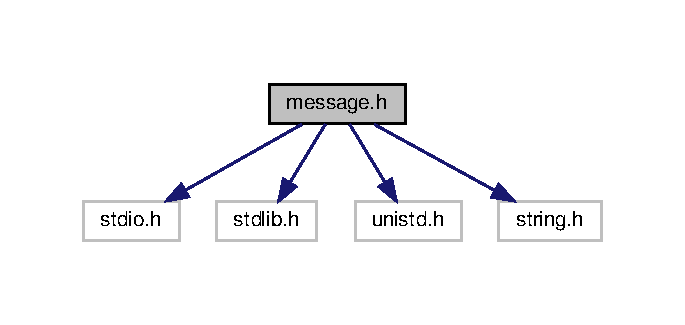
\includegraphics[width=329pt]{message_8h__incl}
\end{center}
\end{figure}
\subsection*{Classes}
\begin{DoxyCompactItemize}
\item 
struct \hyperlink{struct_message_to_mon}{Message\+To\+Mon}
\end{DoxyCompactItemize}
\subsection*{Functions}
\begin{DoxyCompactItemize}
\item 
void \hyperlink{message_8h_a8c768ba3ccfd64ba1e39079c967aff26}{set\+\_\+msg\+To\+Mon\+\_\+header} (\hyperlink{struct_message_to_mon}{Message\+To\+Mon} $\ast$msg, char $\ast$header)
\begin{DoxyCompactList}\small\item\em Set header part of monitor message. \end{DoxyCompactList}\item 
void \hyperlink{message_8h_aa938f8156bfca7379f533b751334ca6f}{set\+\_\+msg\+To\+Mon\+\_\+data} (\hyperlink{struct_message_to_mon}{Message\+To\+Mon} $\ast$msg, void $\ast$data)
\begin{DoxyCompactList}\small\item\em Set data part of monitor message. \end{DoxyCompactList}\item 
void \hyperlink{message_8h_a285193a5a9d3b142f3f1c53c471d3173}{free\+\_\+msg\+To\+Mon\+\_\+data} (\hyperlink{struct_message_to_mon}{Message\+To\+Mon} $\ast$msg)
\begin{DoxyCompactList}\small\item\em Dealocate moemory pointed by data part of message. \end{DoxyCompactList}\item 
void \hyperlink{message_8h_ae409e822d69cee7483a2d41c62698a85}{print\+\_\+msg\+To\+Mon} (\hyperlink{struct_message_to_mon}{Message\+To\+Mon} $\ast$msg)
\begin{DoxyCompactList}\small\item\em Print message, header and data. \end{DoxyCompactList}\end{DoxyCompactItemize}


\subsection{Detailed Description}
Functions for sending message to monitor. 

\begin{DoxyAuthor}{Author}
P\+E.\+Hladik 
\end{DoxyAuthor}
\begin{DoxyVersion}{Version}
1.\+0 
\end{DoxyVersion}
\begin{DoxyDate}{Date}
06/06/2017 
\end{DoxyDate}


\subsection{Function Documentation}
\mbox{\Hypertarget{message_8h_a285193a5a9d3b142f3f1c53c471d3173}\label{message_8h_a285193a5a9d3b142f3f1c53c471d3173}} 
\index{message.\+h@{message.\+h}!free\+\_\+msg\+To\+Mon\+\_\+data@{free\+\_\+msg\+To\+Mon\+\_\+data}}
\index{free\+\_\+msg\+To\+Mon\+\_\+data@{free\+\_\+msg\+To\+Mon\+\_\+data}!message.\+h@{message.\+h}}
\subsubsection{\texorpdfstring{free\+\_\+msg\+To\+Mon\+\_\+data()}{free\_msgToMon\_data()}}
{\footnotesize\ttfamily void free\+\_\+msg\+To\+Mon\+\_\+data (\begin{DoxyParamCaption}\item[{\hyperlink{struct_message_to_mon}{Message\+To\+Mon} $\ast$}]{msg }\end{DoxyParamCaption})}



Dealocate moemory pointed by data part of message. 

\mbox{\Hypertarget{message_8h_ae409e822d69cee7483a2d41c62698a85}\label{message_8h_ae409e822d69cee7483a2d41c62698a85}} 
\index{message.\+h@{message.\+h}!print\+\_\+msg\+To\+Mon@{print\+\_\+msg\+To\+Mon}}
\index{print\+\_\+msg\+To\+Mon@{print\+\_\+msg\+To\+Mon}!message.\+h@{message.\+h}}
\subsubsection{\texorpdfstring{print\+\_\+msg\+To\+Mon()}{print\_msgToMon()}}
{\footnotesize\ttfamily void print\+\_\+msg\+To\+Mon (\begin{DoxyParamCaption}\item[{\hyperlink{struct_message_to_mon}{Message\+To\+Mon} $\ast$}]{msg }\end{DoxyParamCaption})}



Print message, header and data. 

\mbox{\Hypertarget{message_8h_aa938f8156bfca7379f533b751334ca6f}\label{message_8h_aa938f8156bfca7379f533b751334ca6f}} 
\index{message.\+h@{message.\+h}!set\+\_\+msg\+To\+Mon\+\_\+data@{set\+\_\+msg\+To\+Mon\+\_\+data}}
\index{set\+\_\+msg\+To\+Mon\+\_\+data@{set\+\_\+msg\+To\+Mon\+\_\+data}!message.\+h@{message.\+h}}
\subsubsection{\texorpdfstring{set\+\_\+msg\+To\+Mon\+\_\+data()}{set\_msgToMon\_data()}}
{\footnotesize\ttfamily void set\+\_\+msg\+To\+Mon\+\_\+data (\begin{DoxyParamCaption}\item[{\hyperlink{struct_message_to_mon}{Message\+To\+Mon} $\ast$}]{msg,  }\item[{void $\ast$}]{data }\end{DoxyParamCaption})}



Set data part of monitor message. 

\mbox{\Hypertarget{message_8h_a8c768ba3ccfd64ba1e39079c967aff26}\label{message_8h_a8c768ba3ccfd64ba1e39079c967aff26}} 
\index{message.\+h@{message.\+h}!set\+\_\+msg\+To\+Mon\+\_\+header@{set\+\_\+msg\+To\+Mon\+\_\+header}}
\index{set\+\_\+msg\+To\+Mon\+\_\+header@{set\+\_\+msg\+To\+Mon\+\_\+header}!message.\+h@{message.\+h}}
\subsubsection{\texorpdfstring{set\+\_\+msg\+To\+Mon\+\_\+header()}{set\_msgToMon\_header()}}
{\footnotesize\ttfamily void set\+\_\+msg\+To\+Mon\+\_\+header (\begin{DoxyParamCaption}\item[{\hyperlink{struct_message_to_mon}{Message\+To\+Mon} $\ast$}]{msg,  }\item[{char $\ast$}]{header }\end{DoxyParamCaption})}



Set header part of monitor message. 


\hypertarget{monitor_8h}{}\section{monitor.\+h File Reference}
\label{monitor_8h}\index{monitor.\+h@{monitor.\+h}}


Library for sending message to monitor or receiving message.  


{\ttfamily \#include $<$sys/types.\+h$>$}\newline
{\ttfamily \#include $<$sys/socket.\+h$>$}\newline
{\ttfamily \#include $<$netinet/in.\+h$>$}\newline
{\ttfamily \#include $<$arpa/inet.\+h$>$}\newline
{\ttfamily \#include $<$unistd.\+h$>$}\newline
{\ttfamily \#include $<$signal.\+h$>$}\newline
{\ttfamily \#include $<$stdlib.\+h$>$}\newline
{\ttfamily \#include $<$stdio.\+h$>$}\newline
{\ttfamily \#include $<$string.\+h$>$}\newline
{\ttfamily \#include \char`\"{}image.\+h\char`\"{}}\newline
{\ttfamily \#include \char`\"{}definitions.\+h\char`\"{}}\newline
Include dependency graph for monitor.\+h\+:\nopagebreak
\begin{figure}[H]
\begin{center}
\leavevmode
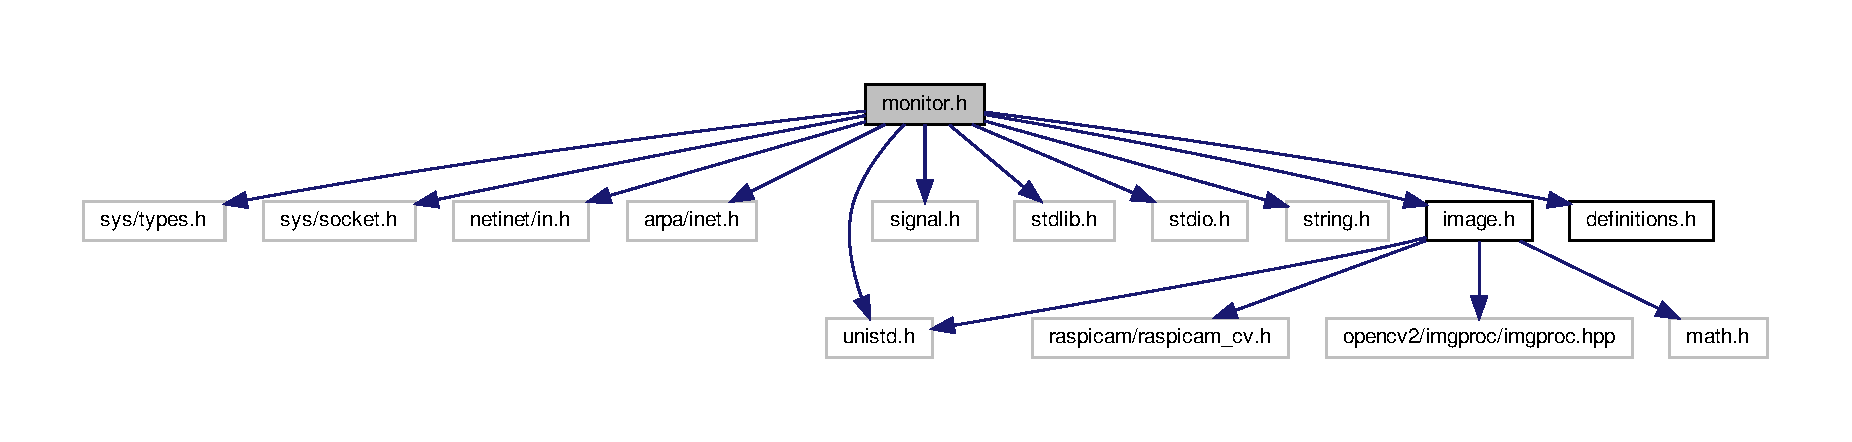
\includegraphics[width=350pt]{monitor_8h__incl}
\end{center}
\end{figure}
\subsection*{Classes}
\begin{DoxyCompactItemize}
\item 
struct \hyperlink{struct_message_from_mon}{Message\+From\+Mon}
\end{DoxyCompactItemize}
\subsection*{Macros}
\begin{DoxyCompactItemize}
\item 
\#define \hyperlink{monitor_8h_ad62b697bd25a71d171db46740aef2830}{H\+E\+A\+D\+E\+R\+\_\+\+S\+T\+M\+\_\+\+I\+M\+A\+GE}~\char`\"{}I\+MG\char`\"{}
\item 
\#define \hyperlink{monitor_8h_a0de226ae5af8b83f3b163ff4413eef95}{H\+E\+A\+D\+E\+R\+\_\+\+S\+T\+M\+\_\+\+B\+AT}~\char`\"{}B\+AT\char`\"{}
\item 
\#define \hyperlink{monitor_8h_a6a07aae2539981459edc8070a0f019db}{H\+E\+A\+D\+E\+R\+\_\+\+S\+T\+M\+\_\+\+P\+OS}~\char`\"{}P\+OS\char`\"{}
\item 
\#define \hyperlink{monitor_8h_ac2e64478522da4e3b45c139c0c72557f}{H\+E\+A\+D\+E\+R\+\_\+\+S\+T\+M\+\_\+\+N\+O\+\_\+\+A\+CK}~\char`\"{}N\+AK\char`\"{}
\item 
\#define \hyperlink{monitor_8h_af2325d19ae9da4310eb608c744149f53}{H\+E\+A\+D\+E\+R\+\_\+\+S\+T\+M\+\_\+\+A\+CK}~\char`\"{}A\+CK\char`\"{}
\item 
\#define \hyperlink{monitor_8h_ac1034bccb09918cccd3ba142377a6788}{H\+E\+A\+D\+E\+R\+\_\+\+S\+T\+M\+\_\+\+M\+ES}~\char`\"{}M\+SG\char`\"{}
\item 
\#define \hyperlink{monitor_8h_afe29ce74d16751828da8aec7e13ad06b}{H\+E\+A\+D\+E\+R\+\_\+\+S\+T\+M\+\_\+\+L\+O\+S\+T\+\_\+\+D\+MB}~\char`\"{}L\+CD\char`\"{}
\item 
\#define \hyperlink{monitor_8h_a980e8f9457e30018fddcd4d997f17a85}{H\+E\+A\+D\+E\+R\+\_\+\+M\+T\+S\+\_\+\+M\+SG}~\char`\"{}M\+SG\char`\"{}
\item 
\#define \hyperlink{monitor_8h_a5ccd30e6502bb94eaa13a597edb1f156}{H\+E\+A\+D\+E\+R\+\_\+\+M\+T\+S\+\_\+\+D\+M\+B\+\_\+\+O\+R\+D\+ER}~\char`\"{}D\+MB\char`\"{}
\item 
\#define \hyperlink{monitor_8h_a0c829d92889c5c9b2d485964ce933fab}{H\+E\+A\+D\+E\+R\+\_\+\+M\+T\+S\+\_\+\+C\+O\+M\+\_\+\+D\+MB}~\char`\"{}C\+OM\char`\"{}
\item 
\#define \hyperlink{monitor_8h_a91e2658cf20010646211ba748885c180}{H\+E\+A\+D\+E\+R\+\_\+\+M\+T\+S\+\_\+\+C\+A\+M\+E\+RA}~\char`\"{}C\+AM\char`\"{}
\item 
\#define \hyperlink{monitor_8h_a2be30c9a3e65eaf5502b8542a6ac6259}{H\+E\+A\+D\+E\+R\+\_\+\+M\+T\+S\+\_\+\+S\+T\+OP}~\char`\"{}S\+TO\char`\"{}
\item 
\#define \hyperlink{monitor_8h_a26769957ec1a2beaf223f33b66ee64ab}{I\+N\+V\+A\+L\+I\+D\+\_\+\+S\+O\+C\+K\+ET}~-\/1
\item 
\#define \hyperlink{monitor_8h_a633b0396ff93d336a088412a190a5072}{S\+O\+C\+K\+E\+T\+\_\+\+E\+R\+R\+OR}~-\/1
\item 
\#define \hyperlink{monitor_8h_a16b710f592bf8f7900666392adc444dc}{D\+E\+F\+A\+U\+L\+T\+\_\+\+P\+O\+RT}~8080
\item 
\#define \hyperlink{monitor_8h_a939612a13947b5bb9fc848e3222a231d}{D\+E\+F\+A\+U\+L\+T\+\_\+\+P\+A\+R\+I\+TY}~0
\item 
\#define \hyperlink{monitor_8h_ab3be9ae187e8b98bb000ca0bca68e982}{D\+E\+T\+E\+C\+T\+\_\+\+A\+R\+E\+NA}~(1)
\item 
\#define \hyperlink{monitor_8h_a22d20ac264e03c59d6941cb11386aa89}{C\+H\+E\+C\+K\+\_\+\+A\+R\+E\+NA}~(2)
\item 
\#define \hyperlink{monitor_8h_a1d58e03abc2a587c7f0a0665c94c0e68}{N\+O\+\_\+\+A\+R\+E\+NA}~(3)
\item 
\#define \hyperlink{monitor_8h_a2c47b710f0858fe41c544517c6b2a2fd}{D\+E\+F\+A\+U\+L\+T\+\_\+\+N\+O\+D\+E\+J\+S\+\_\+\+P\+A\+TH}~\char`\"{}/usr/bin/nodejs\char`\"{}
\item 
\#define \hyperlink{monitor_8h_af533d8bd7d6a1d9f9efba3b259280e32}{D\+E\+F\+A\+U\+L\+T\+\_\+\+I\+N\+T\+E\+R\+F\+A\+C\+E\+\_\+\+F\+I\+LE}~\char`\"{}./interface.\+js\char`\"{}
\item 
\#define \hyperlink{monitor_8h_ab6b45251e218af8f09c5d627b5262398}{closesocket}(param)~close(param)
\end{DoxyCompactItemize}
\subsection*{Typedefs}
\begin{DoxyCompactItemize}
\item 
typedef int \hyperlink{monitor_8h_a8dc8083897335125630f1af5dafd5831}{S\+O\+C\+K\+ET}
\item 
typedef struct sockaddr\+\_\+in \hyperlink{monitor_8h_a29046dc0232f0e5c70adbc25090d77b8}{S\+O\+C\+K\+A\+D\+D\+R\+\_\+\+IN}
\item 
typedef struct sockaddr \hyperlink{monitor_8h_ae334b73cedf7204187dce3f817576009}{S\+O\+C\+K\+A\+D\+DR}
\end{DoxyCompactItemize}
\subsection*{Functions}
\begin{DoxyCompactItemize}
\item 
int \hyperlink{monitor_8h_ac3d876b96642b6ee46f6a96b7ffcb864}{send\+\_\+message\+\_\+to\+\_\+monitor} (const char $\ast$type\+Message, const void $\ast$data=N\+U\+LL)
\begin{DoxyCompactList}\small\item\em Envoi d\textquotesingle{}un message vers l\textquotesingle{}interface graphique. \end{DoxyCompactList}\item 
int \hyperlink{monitor_8h_a61eca0d5b49118350db39583e1bd1032}{receive\+\_\+message\+\_\+from\+\_\+monitor} (char $\ast$type\+Message, char $\ast$data)
\begin{DoxyCompactList}\small\item\em Réception d\textquotesingle{}un message. La fonction est bloquante et retourne par référence le type de message reçu (D\+MB pour un ordre au robot, A\+RN pour la détection des arènes et P\+OS pour un calcul de position) ainsi que les données associées. \end{DoxyCompactList}\end{DoxyCompactItemize}


\subsection{Detailed Description}
Library for sending message to monitor or receiving message. 

\begin{DoxyAuthor}{Author}
L.\+senaneuch 
\end{DoxyAuthor}
\begin{DoxyVersion}{Version}
1.\+0 
\end{DoxyVersion}
\begin{DoxyDate}{Date}
06/06/2017 
\end{DoxyDate}


\subsection{Macro Definition Documentation}
\mbox{\Hypertarget{monitor_8h_a22d20ac264e03c59d6941cb11386aa89}\label{monitor_8h_a22d20ac264e03c59d6941cb11386aa89}} 
\index{monitor.\+h@{monitor.\+h}!C\+H\+E\+C\+K\+\_\+\+A\+R\+E\+NA@{C\+H\+E\+C\+K\+\_\+\+A\+R\+E\+NA}}
\index{C\+H\+E\+C\+K\+\_\+\+A\+R\+E\+NA@{C\+H\+E\+C\+K\+\_\+\+A\+R\+E\+NA}!monitor.\+h@{monitor.\+h}}
\subsubsection{\texorpdfstring{C\+H\+E\+C\+K\+\_\+\+A\+R\+E\+NA}{CHECK\_ARENA}}
{\footnotesize\ttfamily \#define C\+H\+E\+C\+K\+\_\+\+A\+R\+E\+NA~(2)}



Definition at line 62 of file monitor.\+h.

\mbox{\Hypertarget{monitor_8h_ab6b45251e218af8f09c5d627b5262398}\label{monitor_8h_ab6b45251e218af8f09c5d627b5262398}} 
\index{monitor.\+h@{monitor.\+h}!closesocket@{closesocket}}
\index{closesocket@{closesocket}!monitor.\+h@{monitor.\+h}}
\subsubsection{\texorpdfstring{closesocket}{closesocket}}
{\footnotesize\ttfamily \#define closesocket(\begin{DoxyParamCaption}\item[{}]{param }\end{DoxyParamCaption})~close(param)}



Definition at line 68 of file monitor.\+h.

\mbox{\Hypertarget{monitor_8h_af533d8bd7d6a1d9f9efba3b259280e32}\label{monitor_8h_af533d8bd7d6a1d9f9efba3b259280e32}} 
\index{monitor.\+h@{monitor.\+h}!D\+E\+F\+A\+U\+L\+T\+\_\+\+I\+N\+T\+E\+R\+F\+A\+C\+E\+\_\+\+F\+I\+LE@{D\+E\+F\+A\+U\+L\+T\+\_\+\+I\+N\+T\+E\+R\+F\+A\+C\+E\+\_\+\+F\+I\+LE}}
\index{D\+E\+F\+A\+U\+L\+T\+\_\+\+I\+N\+T\+E\+R\+F\+A\+C\+E\+\_\+\+F\+I\+LE@{D\+E\+F\+A\+U\+L\+T\+\_\+\+I\+N\+T\+E\+R\+F\+A\+C\+E\+\_\+\+F\+I\+LE}!monitor.\+h@{monitor.\+h}}
\subsubsection{\texorpdfstring{D\+E\+F\+A\+U\+L\+T\+\_\+\+I\+N\+T\+E\+R\+F\+A\+C\+E\+\_\+\+F\+I\+LE}{DEFAULT\_INTERFACE\_FILE}}
{\footnotesize\ttfamily \#define D\+E\+F\+A\+U\+L\+T\+\_\+\+I\+N\+T\+E\+R\+F\+A\+C\+E\+\_\+\+F\+I\+LE~\char`\"{}./interface.\+js\char`\"{}}



Definition at line 66 of file monitor.\+h.

\mbox{\Hypertarget{monitor_8h_a2c47b710f0858fe41c544517c6b2a2fd}\label{monitor_8h_a2c47b710f0858fe41c544517c6b2a2fd}} 
\index{monitor.\+h@{monitor.\+h}!D\+E\+F\+A\+U\+L\+T\+\_\+\+N\+O\+D\+E\+J\+S\+\_\+\+P\+A\+TH@{D\+E\+F\+A\+U\+L\+T\+\_\+\+N\+O\+D\+E\+J\+S\+\_\+\+P\+A\+TH}}
\index{D\+E\+F\+A\+U\+L\+T\+\_\+\+N\+O\+D\+E\+J\+S\+\_\+\+P\+A\+TH@{D\+E\+F\+A\+U\+L\+T\+\_\+\+N\+O\+D\+E\+J\+S\+\_\+\+P\+A\+TH}!monitor.\+h@{monitor.\+h}}
\subsubsection{\texorpdfstring{D\+E\+F\+A\+U\+L\+T\+\_\+\+N\+O\+D\+E\+J\+S\+\_\+\+P\+A\+TH}{DEFAULT\_NODEJS\_PATH}}
{\footnotesize\ttfamily \#define D\+E\+F\+A\+U\+L\+T\+\_\+\+N\+O\+D\+E\+J\+S\+\_\+\+P\+A\+TH~\char`\"{}/usr/bin/nodejs\char`\"{}}



Definition at line 65 of file monitor.\+h.

\mbox{\Hypertarget{monitor_8h_a939612a13947b5bb9fc848e3222a231d}\label{monitor_8h_a939612a13947b5bb9fc848e3222a231d}} 
\index{monitor.\+h@{monitor.\+h}!D\+E\+F\+A\+U\+L\+T\+\_\+\+P\+A\+R\+I\+TY@{D\+E\+F\+A\+U\+L\+T\+\_\+\+P\+A\+R\+I\+TY}}
\index{D\+E\+F\+A\+U\+L\+T\+\_\+\+P\+A\+R\+I\+TY@{D\+E\+F\+A\+U\+L\+T\+\_\+\+P\+A\+R\+I\+TY}!monitor.\+h@{monitor.\+h}}
\subsubsection{\texorpdfstring{D\+E\+F\+A\+U\+L\+T\+\_\+\+P\+A\+R\+I\+TY}{DEFAULT\_PARITY}}
{\footnotesize\ttfamily \#define D\+E\+F\+A\+U\+L\+T\+\_\+\+P\+A\+R\+I\+TY~0}



Definition at line 59 of file monitor.\+h.

\mbox{\Hypertarget{monitor_8h_a16b710f592bf8f7900666392adc444dc}\label{monitor_8h_a16b710f592bf8f7900666392adc444dc}} 
\index{monitor.\+h@{monitor.\+h}!D\+E\+F\+A\+U\+L\+T\+\_\+\+P\+O\+RT@{D\+E\+F\+A\+U\+L\+T\+\_\+\+P\+O\+RT}}
\index{D\+E\+F\+A\+U\+L\+T\+\_\+\+P\+O\+RT@{D\+E\+F\+A\+U\+L\+T\+\_\+\+P\+O\+RT}!monitor.\+h@{monitor.\+h}}
\subsubsection{\texorpdfstring{D\+E\+F\+A\+U\+L\+T\+\_\+\+P\+O\+RT}{DEFAULT\_PORT}}
{\footnotesize\ttfamily \#define D\+E\+F\+A\+U\+L\+T\+\_\+\+P\+O\+RT~8080}



Definition at line 58 of file monitor.\+h.

\mbox{\Hypertarget{monitor_8h_ab3be9ae187e8b98bb000ca0bca68e982}\label{monitor_8h_ab3be9ae187e8b98bb000ca0bca68e982}} 
\index{monitor.\+h@{monitor.\+h}!D\+E\+T\+E\+C\+T\+\_\+\+A\+R\+E\+NA@{D\+E\+T\+E\+C\+T\+\_\+\+A\+R\+E\+NA}}
\index{D\+E\+T\+E\+C\+T\+\_\+\+A\+R\+E\+NA@{D\+E\+T\+E\+C\+T\+\_\+\+A\+R\+E\+NA}!monitor.\+h@{monitor.\+h}}
\subsubsection{\texorpdfstring{D\+E\+T\+E\+C\+T\+\_\+\+A\+R\+E\+NA}{DETECT\_ARENA}}
{\footnotesize\ttfamily \#define D\+E\+T\+E\+C\+T\+\_\+\+A\+R\+E\+NA~(1)}



Definition at line 61 of file monitor.\+h.

\mbox{\Hypertarget{monitor_8h_a91e2658cf20010646211ba748885c180}\label{monitor_8h_a91e2658cf20010646211ba748885c180}} 
\index{monitor.\+h@{monitor.\+h}!H\+E\+A\+D\+E\+R\+\_\+\+M\+T\+S\+\_\+\+C\+A\+M\+E\+RA@{H\+E\+A\+D\+E\+R\+\_\+\+M\+T\+S\+\_\+\+C\+A\+M\+E\+RA}}
\index{H\+E\+A\+D\+E\+R\+\_\+\+M\+T\+S\+\_\+\+C\+A\+M\+E\+RA@{H\+E\+A\+D\+E\+R\+\_\+\+M\+T\+S\+\_\+\+C\+A\+M\+E\+RA}!monitor.\+h@{monitor.\+h}}
\subsubsection{\texorpdfstring{H\+E\+A\+D\+E\+R\+\_\+\+M\+T\+S\+\_\+\+C\+A\+M\+E\+RA}{HEADER\_MTS\_CAMERA}}
{\footnotesize\ttfamily \#define H\+E\+A\+D\+E\+R\+\_\+\+M\+T\+S\+\_\+\+C\+A\+M\+E\+RA~\char`\"{}C\+AM\char`\"{}}



Definition at line 52 of file monitor.\+h.

\mbox{\Hypertarget{monitor_8h_a0c829d92889c5c9b2d485964ce933fab}\label{monitor_8h_a0c829d92889c5c9b2d485964ce933fab}} 
\index{monitor.\+h@{monitor.\+h}!H\+E\+A\+D\+E\+R\+\_\+\+M\+T\+S\+\_\+\+C\+O\+M\+\_\+\+D\+MB@{H\+E\+A\+D\+E\+R\+\_\+\+M\+T\+S\+\_\+\+C\+O\+M\+\_\+\+D\+MB}}
\index{H\+E\+A\+D\+E\+R\+\_\+\+M\+T\+S\+\_\+\+C\+O\+M\+\_\+\+D\+MB@{H\+E\+A\+D\+E\+R\+\_\+\+M\+T\+S\+\_\+\+C\+O\+M\+\_\+\+D\+MB}!monitor.\+h@{monitor.\+h}}
\subsubsection{\texorpdfstring{H\+E\+A\+D\+E\+R\+\_\+\+M\+T\+S\+\_\+\+C\+O\+M\+\_\+\+D\+MB}{HEADER\_MTS\_COM\_DMB}}
{\footnotesize\ttfamily \#define H\+E\+A\+D\+E\+R\+\_\+\+M\+T\+S\+\_\+\+C\+O\+M\+\_\+\+D\+MB~\char`\"{}C\+OM\char`\"{}}



Definition at line 51 of file monitor.\+h.

\mbox{\Hypertarget{monitor_8h_a5ccd30e6502bb94eaa13a597edb1f156}\label{monitor_8h_a5ccd30e6502bb94eaa13a597edb1f156}} 
\index{monitor.\+h@{monitor.\+h}!H\+E\+A\+D\+E\+R\+\_\+\+M\+T\+S\+\_\+\+D\+M\+B\+\_\+\+O\+R\+D\+ER@{H\+E\+A\+D\+E\+R\+\_\+\+M\+T\+S\+\_\+\+D\+M\+B\+\_\+\+O\+R\+D\+ER}}
\index{H\+E\+A\+D\+E\+R\+\_\+\+M\+T\+S\+\_\+\+D\+M\+B\+\_\+\+O\+R\+D\+ER@{H\+E\+A\+D\+E\+R\+\_\+\+M\+T\+S\+\_\+\+D\+M\+B\+\_\+\+O\+R\+D\+ER}!monitor.\+h@{monitor.\+h}}
\subsubsection{\texorpdfstring{H\+E\+A\+D\+E\+R\+\_\+\+M\+T\+S\+\_\+\+D\+M\+B\+\_\+\+O\+R\+D\+ER}{HEADER\_MTS\_DMB\_ORDER}}
{\footnotesize\ttfamily \#define H\+E\+A\+D\+E\+R\+\_\+\+M\+T\+S\+\_\+\+D\+M\+B\+\_\+\+O\+R\+D\+ER~\char`\"{}D\+MB\char`\"{}}



Definition at line 50 of file monitor.\+h.

\mbox{\Hypertarget{monitor_8h_a980e8f9457e30018fddcd4d997f17a85}\label{monitor_8h_a980e8f9457e30018fddcd4d997f17a85}} 
\index{monitor.\+h@{monitor.\+h}!H\+E\+A\+D\+E\+R\+\_\+\+M\+T\+S\+\_\+\+M\+SG@{H\+E\+A\+D\+E\+R\+\_\+\+M\+T\+S\+\_\+\+M\+SG}}
\index{H\+E\+A\+D\+E\+R\+\_\+\+M\+T\+S\+\_\+\+M\+SG@{H\+E\+A\+D\+E\+R\+\_\+\+M\+T\+S\+\_\+\+M\+SG}!monitor.\+h@{monitor.\+h}}
\subsubsection{\texorpdfstring{H\+E\+A\+D\+E\+R\+\_\+\+M\+T\+S\+\_\+\+M\+SG}{HEADER\_MTS\_MSG}}
{\footnotesize\ttfamily \#define H\+E\+A\+D\+E\+R\+\_\+\+M\+T\+S\+\_\+\+M\+SG~\char`\"{}M\+SG\char`\"{}}



Definition at line 49 of file monitor.\+h.

\mbox{\Hypertarget{monitor_8h_a2be30c9a3e65eaf5502b8542a6ac6259}\label{monitor_8h_a2be30c9a3e65eaf5502b8542a6ac6259}} 
\index{monitor.\+h@{monitor.\+h}!H\+E\+A\+D\+E\+R\+\_\+\+M\+T\+S\+\_\+\+S\+T\+OP@{H\+E\+A\+D\+E\+R\+\_\+\+M\+T\+S\+\_\+\+S\+T\+OP}}
\index{H\+E\+A\+D\+E\+R\+\_\+\+M\+T\+S\+\_\+\+S\+T\+OP@{H\+E\+A\+D\+E\+R\+\_\+\+M\+T\+S\+\_\+\+S\+T\+OP}!monitor.\+h@{monitor.\+h}}
\subsubsection{\texorpdfstring{H\+E\+A\+D\+E\+R\+\_\+\+M\+T\+S\+\_\+\+S\+T\+OP}{HEADER\_MTS\_STOP}}
{\footnotesize\ttfamily \#define H\+E\+A\+D\+E\+R\+\_\+\+M\+T\+S\+\_\+\+S\+T\+OP~\char`\"{}S\+TO\char`\"{}}



Definition at line 53 of file monitor.\+h.

\mbox{\Hypertarget{monitor_8h_af2325d19ae9da4310eb608c744149f53}\label{monitor_8h_af2325d19ae9da4310eb608c744149f53}} 
\index{monitor.\+h@{monitor.\+h}!H\+E\+A\+D\+E\+R\+\_\+\+S\+T\+M\+\_\+\+A\+CK@{H\+E\+A\+D\+E\+R\+\_\+\+S\+T\+M\+\_\+\+A\+CK}}
\index{H\+E\+A\+D\+E\+R\+\_\+\+S\+T\+M\+\_\+\+A\+CK@{H\+E\+A\+D\+E\+R\+\_\+\+S\+T\+M\+\_\+\+A\+CK}!monitor.\+h@{monitor.\+h}}
\subsubsection{\texorpdfstring{H\+E\+A\+D\+E\+R\+\_\+\+S\+T\+M\+\_\+\+A\+CK}{HEADER\_STM\_ACK}}
{\footnotesize\ttfamily \#define H\+E\+A\+D\+E\+R\+\_\+\+S\+T\+M\+\_\+\+A\+CK~\char`\"{}A\+CK\char`\"{}}



Definition at line 45 of file monitor.\+h.

\mbox{\Hypertarget{monitor_8h_a0de226ae5af8b83f3b163ff4413eef95}\label{monitor_8h_a0de226ae5af8b83f3b163ff4413eef95}} 
\index{monitor.\+h@{monitor.\+h}!H\+E\+A\+D\+E\+R\+\_\+\+S\+T\+M\+\_\+\+B\+AT@{H\+E\+A\+D\+E\+R\+\_\+\+S\+T\+M\+\_\+\+B\+AT}}
\index{H\+E\+A\+D\+E\+R\+\_\+\+S\+T\+M\+\_\+\+B\+AT@{H\+E\+A\+D\+E\+R\+\_\+\+S\+T\+M\+\_\+\+B\+AT}!monitor.\+h@{monitor.\+h}}
\subsubsection{\texorpdfstring{H\+E\+A\+D\+E\+R\+\_\+\+S\+T\+M\+\_\+\+B\+AT}{HEADER\_STM\_BAT}}
{\footnotesize\ttfamily \#define H\+E\+A\+D\+E\+R\+\_\+\+S\+T\+M\+\_\+\+B\+AT~\char`\"{}B\+AT\char`\"{}}



Definition at line 42 of file monitor.\+h.

\mbox{\Hypertarget{monitor_8h_ad62b697bd25a71d171db46740aef2830}\label{monitor_8h_ad62b697bd25a71d171db46740aef2830}} 
\index{monitor.\+h@{monitor.\+h}!H\+E\+A\+D\+E\+R\+\_\+\+S\+T\+M\+\_\+\+I\+M\+A\+GE@{H\+E\+A\+D\+E\+R\+\_\+\+S\+T\+M\+\_\+\+I\+M\+A\+GE}}
\index{H\+E\+A\+D\+E\+R\+\_\+\+S\+T\+M\+\_\+\+I\+M\+A\+GE@{H\+E\+A\+D\+E\+R\+\_\+\+S\+T\+M\+\_\+\+I\+M\+A\+GE}!monitor.\+h@{monitor.\+h}}
\subsubsection{\texorpdfstring{H\+E\+A\+D\+E\+R\+\_\+\+S\+T\+M\+\_\+\+I\+M\+A\+GE}{HEADER\_STM\_IMAGE}}
{\footnotesize\ttfamily \#define H\+E\+A\+D\+E\+R\+\_\+\+S\+T\+M\+\_\+\+I\+M\+A\+GE~\char`\"{}I\+MG\char`\"{}}



Definition at line 41 of file monitor.\+h.

\mbox{\Hypertarget{monitor_8h_afe29ce74d16751828da8aec7e13ad06b}\label{monitor_8h_afe29ce74d16751828da8aec7e13ad06b}} 
\index{monitor.\+h@{monitor.\+h}!H\+E\+A\+D\+E\+R\+\_\+\+S\+T\+M\+\_\+\+L\+O\+S\+T\+\_\+\+D\+MB@{H\+E\+A\+D\+E\+R\+\_\+\+S\+T\+M\+\_\+\+L\+O\+S\+T\+\_\+\+D\+MB}}
\index{H\+E\+A\+D\+E\+R\+\_\+\+S\+T\+M\+\_\+\+L\+O\+S\+T\+\_\+\+D\+MB@{H\+E\+A\+D\+E\+R\+\_\+\+S\+T\+M\+\_\+\+L\+O\+S\+T\+\_\+\+D\+MB}!monitor.\+h@{monitor.\+h}}
\subsubsection{\texorpdfstring{H\+E\+A\+D\+E\+R\+\_\+\+S\+T\+M\+\_\+\+L\+O\+S\+T\+\_\+\+D\+MB}{HEADER\_STM\_LOST\_DMB}}
{\footnotesize\ttfamily \#define H\+E\+A\+D\+E\+R\+\_\+\+S\+T\+M\+\_\+\+L\+O\+S\+T\+\_\+\+D\+MB~\char`\"{}L\+CD\char`\"{}}



Definition at line 47 of file monitor.\+h.

\mbox{\Hypertarget{monitor_8h_ac1034bccb09918cccd3ba142377a6788}\label{monitor_8h_ac1034bccb09918cccd3ba142377a6788}} 
\index{monitor.\+h@{monitor.\+h}!H\+E\+A\+D\+E\+R\+\_\+\+S\+T\+M\+\_\+\+M\+ES@{H\+E\+A\+D\+E\+R\+\_\+\+S\+T\+M\+\_\+\+M\+ES}}
\index{H\+E\+A\+D\+E\+R\+\_\+\+S\+T\+M\+\_\+\+M\+ES@{H\+E\+A\+D\+E\+R\+\_\+\+S\+T\+M\+\_\+\+M\+ES}!monitor.\+h@{monitor.\+h}}
\subsubsection{\texorpdfstring{H\+E\+A\+D\+E\+R\+\_\+\+S\+T\+M\+\_\+\+M\+ES}{HEADER\_STM\_MES}}
{\footnotesize\ttfamily \#define H\+E\+A\+D\+E\+R\+\_\+\+S\+T\+M\+\_\+\+M\+ES~\char`\"{}M\+SG\char`\"{}}



Definition at line 46 of file monitor.\+h.

\mbox{\Hypertarget{monitor_8h_ac2e64478522da4e3b45c139c0c72557f}\label{monitor_8h_ac2e64478522da4e3b45c139c0c72557f}} 
\index{monitor.\+h@{monitor.\+h}!H\+E\+A\+D\+E\+R\+\_\+\+S\+T\+M\+\_\+\+N\+O\+\_\+\+A\+CK@{H\+E\+A\+D\+E\+R\+\_\+\+S\+T\+M\+\_\+\+N\+O\+\_\+\+A\+CK}}
\index{H\+E\+A\+D\+E\+R\+\_\+\+S\+T\+M\+\_\+\+N\+O\+\_\+\+A\+CK@{H\+E\+A\+D\+E\+R\+\_\+\+S\+T\+M\+\_\+\+N\+O\+\_\+\+A\+CK}!monitor.\+h@{monitor.\+h}}
\subsubsection{\texorpdfstring{H\+E\+A\+D\+E\+R\+\_\+\+S\+T\+M\+\_\+\+N\+O\+\_\+\+A\+CK}{HEADER\_STM\_NO\_ACK}}
{\footnotesize\ttfamily \#define H\+E\+A\+D\+E\+R\+\_\+\+S\+T\+M\+\_\+\+N\+O\+\_\+\+A\+CK~\char`\"{}N\+AK\char`\"{}}



Definition at line 44 of file monitor.\+h.

\mbox{\Hypertarget{monitor_8h_a6a07aae2539981459edc8070a0f019db}\label{monitor_8h_a6a07aae2539981459edc8070a0f019db}} 
\index{monitor.\+h@{monitor.\+h}!H\+E\+A\+D\+E\+R\+\_\+\+S\+T\+M\+\_\+\+P\+OS@{H\+E\+A\+D\+E\+R\+\_\+\+S\+T\+M\+\_\+\+P\+OS}}
\index{H\+E\+A\+D\+E\+R\+\_\+\+S\+T\+M\+\_\+\+P\+OS@{H\+E\+A\+D\+E\+R\+\_\+\+S\+T\+M\+\_\+\+P\+OS}!monitor.\+h@{monitor.\+h}}
\subsubsection{\texorpdfstring{H\+E\+A\+D\+E\+R\+\_\+\+S\+T\+M\+\_\+\+P\+OS}{HEADER\_STM\_POS}}
{\footnotesize\ttfamily \#define H\+E\+A\+D\+E\+R\+\_\+\+S\+T\+M\+\_\+\+P\+OS~\char`\"{}P\+OS\char`\"{}}



Definition at line 43 of file monitor.\+h.

\mbox{\Hypertarget{monitor_8h_a26769957ec1a2beaf223f33b66ee64ab}\label{monitor_8h_a26769957ec1a2beaf223f33b66ee64ab}} 
\index{monitor.\+h@{monitor.\+h}!I\+N\+V\+A\+L\+I\+D\+\_\+\+S\+O\+C\+K\+ET@{I\+N\+V\+A\+L\+I\+D\+\_\+\+S\+O\+C\+K\+ET}}
\index{I\+N\+V\+A\+L\+I\+D\+\_\+\+S\+O\+C\+K\+ET@{I\+N\+V\+A\+L\+I\+D\+\_\+\+S\+O\+C\+K\+ET}!monitor.\+h@{monitor.\+h}}
\subsubsection{\texorpdfstring{I\+N\+V\+A\+L\+I\+D\+\_\+\+S\+O\+C\+K\+ET}{INVALID\_SOCKET}}
{\footnotesize\ttfamily \#define I\+N\+V\+A\+L\+I\+D\+\_\+\+S\+O\+C\+K\+ET~-\/1}



Definition at line 55 of file monitor.\+h.

\mbox{\Hypertarget{monitor_8h_a1d58e03abc2a587c7f0a0665c94c0e68}\label{monitor_8h_a1d58e03abc2a587c7f0a0665c94c0e68}} 
\index{monitor.\+h@{monitor.\+h}!N\+O\+\_\+\+A\+R\+E\+NA@{N\+O\+\_\+\+A\+R\+E\+NA}}
\index{N\+O\+\_\+\+A\+R\+E\+NA@{N\+O\+\_\+\+A\+R\+E\+NA}!monitor.\+h@{monitor.\+h}}
\subsubsection{\texorpdfstring{N\+O\+\_\+\+A\+R\+E\+NA}{NO\_ARENA}}
{\footnotesize\ttfamily \#define N\+O\+\_\+\+A\+R\+E\+NA~(3)}



Definition at line 63 of file monitor.\+h.

\mbox{\Hypertarget{monitor_8h_a633b0396ff93d336a088412a190a5072}\label{monitor_8h_a633b0396ff93d336a088412a190a5072}} 
\index{monitor.\+h@{monitor.\+h}!S\+O\+C\+K\+E\+T\+\_\+\+E\+R\+R\+OR@{S\+O\+C\+K\+E\+T\+\_\+\+E\+R\+R\+OR}}
\index{S\+O\+C\+K\+E\+T\+\_\+\+E\+R\+R\+OR@{S\+O\+C\+K\+E\+T\+\_\+\+E\+R\+R\+OR}!monitor.\+h@{monitor.\+h}}
\subsubsection{\texorpdfstring{S\+O\+C\+K\+E\+T\+\_\+\+E\+R\+R\+OR}{SOCKET\_ERROR}}
{\footnotesize\ttfamily \#define S\+O\+C\+K\+E\+T\+\_\+\+E\+R\+R\+OR~-\/1}



Definition at line 56 of file monitor.\+h.



\subsection{Typedef Documentation}
\mbox{\Hypertarget{monitor_8h_ae334b73cedf7204187dce3f817576009}\label{monitor_8h_ae334b73cedf7204187dce3f817576009}} 
\index{monitor.\+h@{monitor.\+h}!S\+O\+C\+K\+A\+D\+DR@{S\+O\+C\+K\+A\+D\+DR}}
\index{S\+O\+C\+K\+A\+D\+DR@{S\+O\+C\+K\+A\+D\+DR}!monitor.\+h@{monitor.\+h}}
\subsubsection{\texorpdfstring{S\+O\+C\+K\+A\+D\+DR}{SOCKADDR}}
{\footnotesize\ttfamily typedef struct sockaddr \hyperlink{monitor_8h_ae334b73cedf7204187dce3f817576009}{S\+O\+C\+K\+A\+D\+DR}}



Definition at line 72 of file monitor.\+h.

\mbox{\Hypertarget{monitor_8h_a29046dc0232f0e5c70adbc25090d77b8}\label{monitor_8h_a29046dc0232f0e5c70adbc25090d77b8}} 
\index{monitor.\+h@{monitor.\+h}!S\+O\+C\+K\+A\+D\+D\+R\+\_\+\+IN@{S\+O\+C\+K\+A\+D\+D\+R\+\_\+\+IN}}
\index{S\+O\+C\+K\+A\+D\+D\+R\+\_\+\+IN@{S\+O\+C\+K\+A\+D\+D\+R\+\_\+\+IN}!monitor.\+h@{monitor.\+h}}
\subsubsection{\texorpdfstring{S\+O\+C\+K\+A\+D\+D\+R\+\_\+\+IN}{SOCKADDR\_IN}}
{\footnotesize\ttfamily typedef struct sockaddr\+\_\+in \hyperlink{monitor_8h_a29046dc0232f0e5c70adbc25090d77b8}{S\+O\+C\+K\+A\+D\+D\+R\+\_\+\+IN}}



Definition at line 71 of file monitor.\+h.

\mbox{\Hypertarget{monitor_8h_a8dc8083897335125630f1af5dafd5831}\label{monitor_8h_a8dc8083897335125630f1af5dafd5831}} 
\index{monitor.\+h@{monitor.\+h}!S\+O\+C\+K\+ET@{S\+O\+C\+K\+ET}}
\index{S\+O\+C\+K\+ET@{S\+O\+C\+K\+ET}!monitor.\+h@{monitor.\+h}}
\subsubsection{\texorpdfstring{S\+O\+C\+K\+ET}{SOCKET}}
{\footnotesize\ttfamily typedef int \hyperlink{monitor_8h_a8dc8083897335125630f1af5dafd5831}{S\+O\+C\+K\+ET}}



Definition at line 70 of file monitor.\+h.



\subsection{Function Documentation}
\mbox{\Hypertarget{monitor_8h_a61eca0d5b49118350db39583e1bd1032}\label{monitor_8h_a61eca0d5b49118350db39583e1bd1032}} 
\index{monitor.\+h@{monitor.\+h}!receive\+\_\+message\+\_\+from\+\_\+monitor@{receive\+\_\+message\+\_\+from\+\_\+monitor}}
\index{receive\+\_\+message\+\_\+from\+\_\+monitor@{receive\+\_\+message\+\_\+from\+\_\+monitor}!monitor.\+h@{monitor.\+h}}
\subsubsection{\texorpdfstring{receive\+\_\+message\+\_\+from\+\_\+monitor()}{receive\_message\_from\_monitor()}}
{\footnotesize\ttfamily int receive\+\_\+message\+\_\+from\+\_\+monitor (\begin{DoxyParamCaption}\item[{char $\ast$}]{type\+Message,  }\item[{char $\ast$}]{data }\end{DoxyParamCaption})}



Réception d\textquotesingle{}un message. La fonction est bloquante et retourne par référence le type de message reçu (D\+MB pour un ordre au robot, A\+RN pour la détection des arènes et P\+OS pour un calcul de position) ainsi que les données associées. 


\begin{DoxyParams}{Parameters}
{\em type\+Message} & Type du message reçu \+: D\+MB pour un ordre au robot, A\+RN pour la demande de détection de l\textquotesingle{}arène, P\+OS pour un calcul de position et M\+SG pour un message de l\textquotesingle{}interface \\
\hline
{\em data} & données associées au message reçu. \\
\hline
\end{DoxyParams}
\begin{DoxyReturn}{Returns}
Retourne 0 la taille du message reçu ou une valeur négative si la connexion est perdue. 
\end{DoxyReturn}
\mbox{\Hypertarget{monitor_8h_ac3d876b96642b6ee46f6a96b7ffcb864}\label{monitor_8h_ac3d876b96642b6ee46f6a96b7ffcb864}} 
\index{monitor.\+h@{monitor.\+h}!send\+\_\+message\+\_\+to\+\_\+monitor@{send\+\_\+message\+\_\+to\+\_\+monitor}}
\index{send\+\_\+message\+\_\+to\+\_\+monitor@{send\+\_\+message\+\_\+to\+\_\+monitor}!monitor.\+h@{monitor.\+h}}
\subsubsection{\texorpdfstring{send\+\_\+message\+\_\+to\+\_\+monitor()}{send\_message\_to\_monitor()}}
{\footnotesize\ttfamily int send\+\_\+message\+\_\+to\+\_\+monitor (\begin{DoxyParamCaption}\item[{const char $\ast$}]{type\+Message,  }\item[{const void $\ast$}]{data = {\ttfamily NULL} }\end{DoxyParamCaption})}



Envoi d\textquotesingle{}un message vers l\textquotesingle{}interface graphique. 


\begin{DoxyParams}{Parameters}
{\em type\+Message} & Type du message envoyé. Les valeurs possibles sont I\+MG pour une image, M\+ES pour un message à afficher dans la console, P\+OS pour la position du robot, B\+AT pour une valeur de la batterie et A\+CK pour valider un message de l\textquotesingle{}interface. \\
\hline
{\em data} & données associées au message. Le type de la donnée doit correspondre au message \+: Image pour I\+MG, char $\ast$ M\+ES, \hyperlink{struct_position}{Position} pour P\+OS, char $\ast$ pour B\+AT et rien pour A\+CK. Attention, il n\textquotesingle{}y a aucune vérification a posterio. \\
\hline
\end{DoxyParams}
\begin{DoxyReturn}{Returns}
Retourne 0 si l\textquotesingle{}envoie a bien été réalisé et -\/1 en cas de problème. 
\end{DoxyReturn}

\hypertarget{robot_8h}{}\section{robot.\+h File Reference}
\label{robot_8h}\index{robot.\+h@{robot.\+h}}


Fonctions for communicating with robot.  


{\ttfamily \#include $<$stdio.\+h$>$}\newline
{\ttfamily \#include $<$unistd.\+h$>$}\newline
{\ttfamily \#include $<$fcntl.\+h$>$}\newline
{\ttfamily \#include $<$termios.\+h$>$}\newline
{\ttfamily \#include $<$string.\+h$>$}\newline
{\ttfamily \#include $<$stdlib.\+h$>$}\newline
{\ttfamily \#include \char`\"{}definitions.\+h\char`\"{}}\newline
Include dependency graph for robot.\+h\+:\nopagebreak
\begin{figure}[H]
\begin{center}
\leavevmode
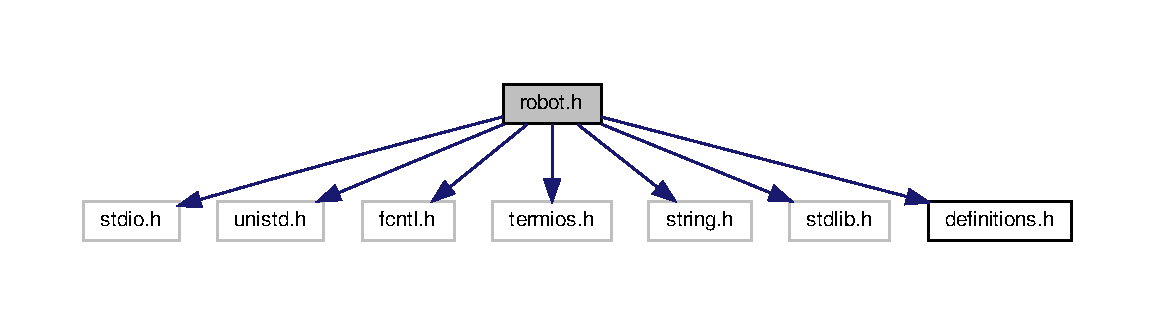
\includegraphics[width=350pt]{robot_8h__incl}
\end{center}
\end{figure}
\subsection*{Classes}
\begin{DoxyCompactItemize}
\item 
struct \hyperlink{struct_message_to_robot}{Message\+To\+Robot}
\end{DoxyCompactItemize}
\subsection*{Macros}
\begin{DoxyCompactItemize}
\item 
\#define \hyperlink{robot_8h_a32c8768c18732c59b503f8ee7515a693}{serial\+Port}~\char`\"{}/dev/tty\+S0\char`\"{}
\end{DoxyCompactItemize}
\subsection*{Functions}
\begin{DoxyCompactItemize}
\item 
int \hyperlink{robot_8h_a0e70fa821a04d349552b8bd54f6935db}{open\+\_\+communication\+\_\+robot} (const char $\ast$path=\hyperlink{robot_8h_a32c8768c18732c59b503f8ee7515a693}{serial\+Port})
\begin{DoxyCompactList}\small\item\em Ouvre la communication avec le robot. \end{DoxyCompactList}\item 
int \hyperlink{robot_8h_a3fbce7530a62f9287f8a3b85b9c7e4d7}{close\+\_\+communication\+\_\+robot} (void)
\begin{DoxyCompactList}\small\item\em Ferme la communication avec le robot. \end{DoxyCompactList}\item 
int \hyperlink{robot_8h_abe88fd581be321a9d86ae7063abd2f65}{send\+\_\+command\+\_\+to\+\_\+robot} (char cmd, const char $\ast$arg=N\+U\+LL)
\begin{DoxyCompactList}\small\item\em Envoi une commande au robot et attends sa réponse. \end{DoxyCompactList}\end{DoxyCompactItemize}


\subsection{Detailed Description}
Fonctions for communicating with robot. 

\begin{DoxyAuthor}{Author}
L.\+Senaneuch 
\end{DoxyAuthor}
\begin{DoxyVersion}{Version}
1.\+0 
\end{DoxyVersion}
\begin{DoxyDate}{Date}
06/06/2017 
\end{DoxyDate}


\subsection{Macro Definition Documentation}
\mbox{\Hypertarget{robot_8h_a32c8768c18732c59b503f8ee7515a693}\label{robot_8h_a32c8768c18732c59b503f8ee7515a693}} 
\index{robot.\+h@{robot.\+h}!serial\+Port@{serial\+Port}}
\index{serial\+Port@{serial\+Port}!robot.\+h@{robot.\+h}}
\subsubsection{\texorpdfstring{serial\+Port}{serialPort}}
{\footnotesize\ttfamily \#define serial\+Port~\char`\"{}/dev/tty\+S0\char`\"{}}



Definition at line 40 of file robot.\+h.



\subsection{Function Documentation}
\mbox{\Hypertarget{robot_8h_a3fbce7530a62f9287f8a3b85b9c7e4d7}\label{robot_8h_a3fbce7530a62f9287f8a3b85b9c7e4d7}} 
\index{robot.\+h@{robot.\+h}!close\+\_\+communication\+\_\+robot@{close\+\_\+communication\+\_\+robot}}
\index{close\+\_\+communication\+\_\+robot@{close\+\_\+communication\+\_\+robot}!robot.\+h@{robot.\+h}}
\subsubsection{\texorpdfstring{close\+\_\+communication\+\_\+robot()}{close\_communication\_robot()}}
{\footnotesize\ttfamily int close\+\_\+communication\+\_\+robot (\begin{DoxyParamCaption}\item[{void}]{ }\end{DoxyParamCaption})}



Ferme la communication avec le robot. 

Ferme le descripteur de fichier du port serie contrôlant le robot.

\begin{DoxyReturn}{Returns}
Retourne -\/1 en cas d\textquotesingle{}erreur ou 0 en cas de fermeture effectué 
\end{DoxyReturn}
\mbox{\Hypertarget{robot_8h_a0e70fa821a04d349552b8bd54f6935db}\label{robot_8h_a0e70fa821a04d349552b8bd54f6935db}} 
\index{robot.\+h@{robot.\+h}!open\+\_\+communication\+\_\+robot@{open\+\_\+communication\+\_\+robot}}
\index{open\+\_\+communication\+\_\+robot@{open\+\_\+communication\+\_\+robot}!robot.\+h@{robot.\+h}}
\subsubsection{\texorpdfstring{open\+\_\+communication\+\_\+robot()}{open\_communication\_robot()}}
{\footnotesize\ttfamily int open\+\_\+communication\+\_\+robot (\begin{DoxyParamCaption}\item[{const char $\ast$}]{path = {\ttfamily \hyperlink{robot_8h_a32c8768c18732c59b503f8ee7515a693}{serial\+Port}} }\end{DoxyParamCaption})}



Ouvre la communication avec le robot. 

Ouvre le serial port passé en paramétre. Par defaut cette fonction ouvre le port tty\+SO connecté au module xbee.


\begin{DoxyParams}{Parameters}
{\em path} & Chaine de caractère contenant le path du port serie à ouvrir. \\
\hline
\end{DoxyParams}
\begin{DoxyReturn}{Returns}
Return -\/1 si l\textquotesingle{}ouverture c\textquotesingle{}est mal passé et 0 si le port est ouvert. 
\end{DoxyReturn}
\mbox{\Hypertarget{robot_8h_abe88fd581be321a9d86ae7063abd2f65}\label{robot_8h_abe88fd581be321a9d86ae7063abd2f65}} 
\index{robot.\+h@{robot.\+h}!send\+\_\+command\+\_\+to\+\_\+robot@{send\+\_\+command\+\_\+to\+\_\+robot}}
\index{send\+\_\+command\+\_\+to\+\_\+robot@{send\+\_\+command\+\_\+to\+\_\+robot}!robot.\+h@{robot.\+h}}
\subsubsection{\texorpdfstring{send\+\_\+command\+\_\+to\+\_\+robot()}{send\_command\_to\_robot()}}
{\footnotesize\ttfamily int send\+\_\+command\+\_\+to\+\_\+robot (\begin{DoxyParamCaption}\item[{char}]{cmd,  }\item[{const char $\ast$}]{arg = {\ttfamily NULL} }\end{DoxyParamCaption})}



Envoi une commande au robot et attends sa réponse. 

Envoi une commande au robot en ajoutant le checksum et lis la réponse du robot en verifiant le checksum. Le premier paramétre {\itshape cmd} correspond au type de commande ex \+: P\+I\+NG, S\+E\+T\+M\+O\+VE ... Le second paramétre {\itshape $\ast$arg} correspond aux arguments à la commande ex \+: S\+E\+T\+M\+O\+VE, \char`\"{}100\char`\"{} La fonction retourne un code confirmation transmise par le robot (R\+O\+B\+O\+T\+\_\+\+C\+H\+E\+K\+S\+UM, R\+O\+B\+O\+T\+\_\+\+E\+R\+R\+OR, R\+O\+B\+O\+T\+\_\+\+T\+I\+M\+E\+D\+\_\+\+O\+UT, R\+O\+B\+O\+T\+\_\+\+OK, R\+O\+B\+O\+T\+\_\+\+U\+K\+N\+O\+W\+\_\+\+C\+MD)


\begin{DoxyParams}{Parameters}
{\em cmd} & Entête de la commande \\
\hline
{\em arg} & Argument de la commande \\
\hline
\end{DoxyParams}
\begin{DoxyReturn}{Returns}
Retourne un code confirmation. 
\end{DoxyReturn}

\hypertarget{server_8h}{}\section{server.\+h File Reference}
\label{server_8h}\index{server.\+h@{server.\+h}}


Library for opening a T\+CP server, receiving data and sending message to monitor.  


{\ttfamily \#include \char`\"{}image.\+h\char`\"{}}\newline
Include dependency graph for server.\+h\+:\nopagebreak
\begin{figure}[H]
\begin{center}
\leavevmode
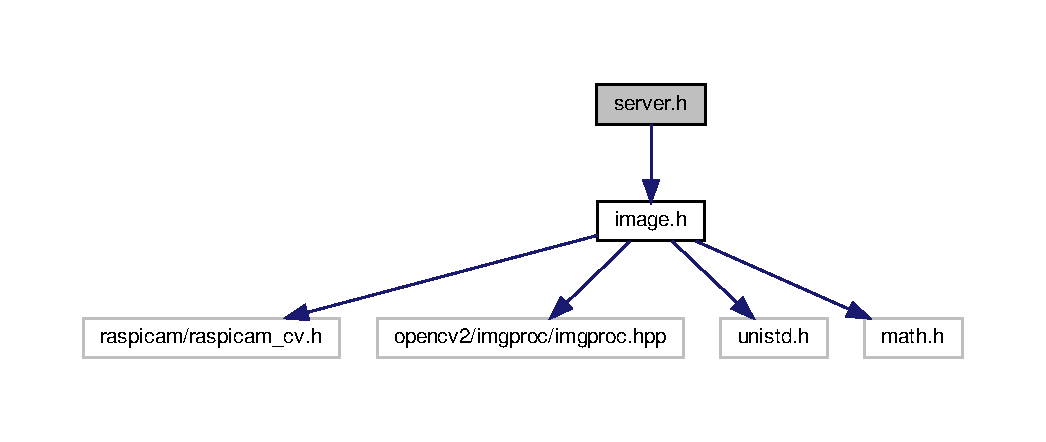
\includegraphics[width=350pt]{server_8h__incl}
\end{center}
\end{figure}
\subsection*{Macros}
\begin{DoxyCompactItemize}
\item 
\#define \hyperlink{server_8h_af257e2a3e091629829857a2eb8931a7a}{D\+E\+F\+A\+U\+L\+T\+\_\+\+S\+E\+R\+V\+E\+R\+\_\+\+P\+O\+RT}~2323
\end{DoxyCompactItemize}
\subsection*{Functions}
\begin{DoxyCompactItemize}
\item 
int \hyperlink{server_8h_a99b54d5b3404766f906f49605a4aa0e3}{open\+Server} (int port)
\begin{DoxyCompactList}\small\item\em Open server port, connect and listen to given port. \end{DoxyCompactList}\item 
int \hyperlink{server_8h_ab65b2df50051036defe0f35366f5a3d6}{close\+Server} ()
\begin{DoxyCompactList}\small\item\em Close server. \end{DoxyCompactList}\item 
int \hyperlink{server_8h_abff9f8e931ecce919588b371dc511857}{accept\+Client} ()
\begin{DoxyCompactList}\small\item\em Wait for a client to connect. \end{DoxyCompactList}\item 
int \hyperlink{server_8h_a8d865d29914b980fd71ed8d347e4ec50}{send\+Data\+To\+Server} (char $\ast$data, int length)
\begin{DoxyCompactList}\small\item\em Send given data to monitor. \end{DoxyCompactList}\item 
int \hyperlink{server_8h_a4c2df7961aa7379ac79d80980a1c537b}{send\+Data\+To\+Server\+For\+Client} (int client, char $\ast$data, int length)
\begin{DoxyCompactList}\small\item\em Send given data to monitor, using specific client ID. \end{DoxyCompactList}\item 
int \hyperlink{server_8h_a8b66a2007f3f9ed8538428a309c9d368}{receive\+Data\+From\+Server} (char $\ast$data, int size)
\begin{DoxyCompactList}\small\item\em Read data from monitor. \end{DoxyCompactList}\item 
int \hyperlink{server_8h_a247e0124af257d0cc7abc25a7c448d1b}{receive\+Data\+From\+Server\+From\+Client} (int client, char $\ast$data, int size)
\begin{DoxyCompactList}\small\item\em Read data from monitor, using specific client ID. \end{DoxyCompactList}\item 
int \hyperlink{server_8h_a51b9372f5467705aa81d76ae034c7628}{send\+Image} (\hyperlink{image_8h_a9ac2855e21920c676a108df386ff9415}{Jpg} $\ast$image)
\begin{DoxyCompactList}\small\item\em Send image to monitor using default client ID. \end{DoxyCompactList}\end{DoxyCompactItemize}


\subsection{Detailed Description}
Library for opening a T\+CP server, receiving data and sending message to monitor. 

\begin{DoxyAuthor}{Author}
P\+E.\+Hladik 
\end{DoxyAuthor}
\begin{DoxyVersion}{Version}
1.\+0 
\end{DoxyVersion}
\begin{DoxyDate}{Date}
06/06/2017 
\end{DoxyDate}


\subsection{Macro Definition Documentation}
\mbox{\Hypertarget{server_8h_af257e2a3e091629829857a2eb8931a7a}\label{server_8h_af257e2a3e091629829857a2eb8931a7a}} 
\index{server.\+h@{server.\+h}!D\+E\+F\+A\+U\+L\+T\+\_\+\+S\+E\+R\+V\+E\+R\+\_\+\+P\+O\+RT@{D\+E\+F\+A\+U\+L\+T\+\_\+\+S\+E\+R\+V\+E\+R\+\_\+\+P\+O\+RT}}
\index{D\+E\+F\+A\+U\+L\+T\+\_\+\+S\+E\+R\+V\+E\+R\+\_\+\+P\+O\+RT@{D\+E\+F\+A\+U\+L\+T\+\_\+\+S\+E\+R\+V\+E\+R\+\_\+\+P\+O\+RT}!server.\+h@{server.\+h}}
\subsubsection{\texorpdfstring{D\+E\+F\+A\+U\+L\+T\+\_\+\+S\+E\+R\+V\+E\+R\+\_\+\+P\+O\+RT}{DEFAULT\_SERVER\_PORT}}
{\footnotesize\ttfamily \#define D\+E\+F\+A\+U\+L\+T\+\_\+\+S\+E\+R\+V\+E\+R\+\_\+\+P\+O\+RT~2323}



Definition at line 30 of file server.\+h.



\subsection{Function Documentation}
\mbox{\Hypertarget{server_8h_abff9f8e931ecce919588b371dc511857}\label{server_8h_abff9f8e931ecce919588b371dc511857}} 
\index{server.\+h@{server.\+h}!accept\+Client@{accept\+Client}}
\index{accept\+Client@{accept\+Client}!server.\+h@{server.\+h}}
\subsubsection{\texorpdfstring{accept\+Client()}{acceptClient()}}
{\footnotesize\ttfamily int accept\+Client (\begin{DoxyParamCaption}{ }\end{DoxyParamCaption})}



Wait for a client to connect. 

\begin{DoxyReturn}{Returns}
Return client Id or -\/1 if it failed 
\end{DoxyReturn}
\mbox{\Hypertarget{server_8h_ab65b2df50051036defe0f35366f5a3d6}\label{server_8h_ab65b2df50051036defe0f35366f5a3d6}} 
\index{server.\+h@{server.\+h}!close\+Server@{close\+Server}}
\index{close\+Server@{close\+Server}!server.\+h@{server.\+h}}
\subsubsection{\texorpdfstring{close\+Server()}{closeServer()}}
{\footnotesize\ttfamily int close\+Server (\begin{DoxyParamCaption}{ }\end{DoxyParamCaption})}



Close server. 

\begin{DoxyReturn}{Returns}
-\/1 if closing failed , 0 otherwise 
\end{DoxyReturn}
\mbox{\Hypertarget{server_8h_a99b54d5b3404766f906f49605a4aa0e3}\label{server_8h_a99b54d5b3404766f906f49605a4aa0e3}} 
\index{server.\+h@{server.\+h}!open\+Server@{open\+Server}}
\index{open\+Server@{open\+Server}!server.\+h@{server.\+h}}
\subsubsection{\texorpdfstring{open\+Server()}{openServer()}}
{\footnotesize\ttfamily int open\+Server (\begin{DoxyParamCaption}\item[{int}]{port }\end{DoxyParamCaption})}



Open server port, connect and listen to given port. 


\begin{DoxyParams}{Parameters}
{\em port} & A valid port number (1024 -\/ 65535) \\
\hline
\end{DoxyParams}
\begin{DoxyReturn}{Returns}
-\/1 if opening failed or the socket number 
\end{DoxyReturn}
\mbox{\Hypertarget{server_8h_a8b66a2007f3f9ed8538428a309c9d368}\label{server_8h_a8b66a2007f3f9ed8538428a309c9d368}} 
\index{server.\+h@{server.\+h}!receive\+Data\+From\+Server@{receive\+Data\+From\+Server}}
\index{receive\+Data\+From\+Server@{receive\+Data\+From\+Server}!server.\+h@{server.\+h}}
\subsubsection{\texorpdfstring{receive\+Data\+From\+Server()}{receiveDataFromServer()}}
{\footnotesize\ttfamily int receive\+Data\+From\+Server (\begin{DoxyParamCaption}\item[{char $\ast$}]{data,  }\item[{int}]{size }\end{DoxyParamCaption})}



Read data from monitor. 

Read, at most, size data from monitor. Data must be a valid pointer to a buffer large enough.


\begin{DoxyParams}{Parameters}
{\em data} & A valid pointer to a buffer \\
\hline
{\em size} & Amount of data to read \\
\hline
\end{DoxyParams}
\begin{DoxyReturn}{Returns}
Return amount of data really received. 0 if communication is broken 
\end{DoxyReturn}
\mbox{\Hypertarget{server_8h_a247e0124af257d0cc7abc25a7c448d1b}\label{server_8h_a247e0124af257d0cc7abc25a7c448d1b}} 
\index{server.\+h@{server.\+h}!receive\+Data\+From\+Server\+From\+Client@{receive\+Data\+From\+Server\+From\+Client}}
\index{receive\+Data\+From\+Server\+From\+Client@{receive\+Data\+From\+Server\+From\+Client}!server.\+h@{server.\+h}}
\subsubsection{\texorpdfstring{receive\+Data\+From\+Server\+From\+Client()}{receiveDataFromServerFromClient()}}
{\footnotesize\ttfamily int receive\+Data\+From\+Server\+From\+Client (\begin{DoxyParamCaption}\item[{int}]{client,  }\item[{char $\ast$}]{data,  }\item[{int}]{size }\end{DoxyParamCaption})}



Read data from monitor, using specific client ID. 

Read, at most, size data from monitor. Data must be a valid pointer to a buffer large enough.


\begin{DoxyParams}{Parameters}
{\em client} & Client Id to receive from \\
\hline
{\em data} & A valid pointer to a buffer \\
\hline
{\em size} & Amount of data to read \\
\hline
\end{DoxyParams}
\begin{DoxyReturn}{Returns}
Return amount of data really received. 0 if communication is broken 
\end{DoxyReturn}
\mbox{\Hypertarget{server_8h_a8d865d29914b980fd71ed8d347e4ec50}\label{server_8h_a8d865d29914b980fd71ed8d347e4ec50}} 
\index{server.\+h@{server.\+h}!send\+Data\+To\+Server@{send\+Data\+To\+Server}}
\index{send\+Data\+To\+Server@{send\+Data\+To\+Server}!server.\+h@{server.\+h}}
\subsubsection{\texorpdfstring{send\+Data\+To\+Server()}{sendDataToServer()}}
{\footnotesize\ttfamily int send\+Data\+To\+Server (\begin{DoxyParamCaption}\item[{char $\ast$}]{data,  }\item[{int}]{length }\end{DoxyParamCaption})}



Send given data to monitor. 

Send given data to monitor using default client ID


\begin{DoxyParams}{Parameters}
{\em data} & A valid pointer to a buffer \\
\hline
{\em length} & Amount of data to send \\
\hline
\end{DoxyParams}
\begin{DoxyReturn}{Returns}
Return amount of data really written. 0 if communication is broken 
\end{DoxyReturn}
\mbox{\Hypertarget{server_8h_a4c2df7961aa7379ac79d80980a1c537b}\label{server_8h_a4c2df7961aa7379ac79d80980a1c537b}} 
\index{server.\+h@{server.\+h}!send\+Data\+To\+Server\+For\+Client@{send\+Data\+To\+Server\+For\+Client}}
\index{send\+Data\+To\+Server\+For\+Client@{send\+Data\+To\+Server\+For\+Client}!server.\+h@{server.\+h}}
\subsubsection{\texorpdfstring{send\+Data\+To\+Server\+For\+Client()}{sendDataToServerForClient()}}
{\footnotesize\ttfamily int send\+Data\+To\+Server\+For\+Client (\begin{DoxyParamCaption}\item[{int}]{client,  }\item[{char $\ast$}]{data,  }\item[{int}]{length }\end{DoxyParamCaption})}



Send given data to monitor, using specific client ID. 

Send given data to monitor using given client ID.


\begin{DoxyParams}{Parameters}
{\em client} & Client Id to send data to \\
\hline
{\em data} & A valid pointer to a buffer \\
\hline
{\em length} & Amount of data to send \\
\hline
\end{DoxyParams}
\begin{DoxyReturn}{Returns}
Return amount of data really written. 0 if communication is broken 
\end{DoxyReturn}
\mbox{\Hypertarget{server_8h_a51b9372f5467705aa81d76ae034c7628}\label{server_8h_a51b9372f5467705aa81d76ae034c7628}} 
\index{server.\+h@{server.\+h}!send\+Image@{send\+Image}}
\index{send\+Image@{send\+Image}!server.\+h@{server.\+h}}
\subsubsection{\texorpdfstring{send\+Image()}{sendImage()}}
{\footnotesize\ttfamily int send\+Image (\begin{DoxyParamCaption}\item[{\hyperlink{image_8h_a9ac2855e21920c676a108df386ff9415}{Jpg} $\ast$}]{image }\end{DoxyParamCaption})}



Send image to monitor using default client ID. 

Convert image to raw data, and add correct header before sending to monitor


\begin{DoxyParams}{Parameters}
{\em image} & An image object after compression \\
\hline
\end{DoxyParams}
\begin{DoxyReturn}{Returns}
Return amount of data really received. 0 if communication is broken 
\end{DoxyReturn}

%--- End generated contents ---

% Index
\backmatter
\newpage
\phantomsection
\clearemptydoublepage
\addcontentsline{toc}{chapter}{Index}
\printindex

\end{document}
